
\documentclass[12pt]{report}
\usepackage[thinc]{esdiff} % for typesettign derivatives
\usepackage{amsthm} % provides an enhanced version of LaTex's \newtheorem command
\usepackage{mdframed} % framed environments that can split at page boundaries
\usepackage{enumitem} % bulletin points or other means of listing things
\usepackage{amssymb} % for AMS symbols
\usepackage{amsmath} % so as to use align
\usepackage{mathrsfs} % for the stylistic L
\usepackage{authblk} % for writing affiliationis
\usepackage{graphicx} % for importing images
\graphicspath{{./images/}} % for the path to images


\theoremstyle{definition}
\mdfdefinestyle{defEnv}{%
  hidealllines=false,
  nobreak=true,
  innertopmargin=-1ex,
}

\pagestyle{headings}
\author{Lectured by Marie-Amelie Lawn, Frank Berkshire}
\title{Calculus, Algebra, and Analysis for JMC}
\affil{Typed by Aris Zhu Yi Qing}
\begin{document}
\maketitle
\tableofcontents

\chapter{Group theory}

Study of the simplest algebraic structure on a set.

\section{Basic Definitions and Examples}

\subsection{Binary operations and groups}

\newmdtheoremenv[style=defEnv]{theorem}{Definition}
\begin{theorem}
    \emph{Set} is a collection of distinct elements. Let $G$ be a set.
    \textbf{\emph{Binary operation on G}} is a function\[
        *: G \times G \rightarrow G \textnormal{(Closure is included)}
    \]
\end{theorem}

\newtheorem{ex}[theorem]{Example}
\begin{ex}
    \;
    
    \begin{itemize}
        \item $(\mathbb{N}, +), (\mathbb{Z}, +), (\mathbb{R}, \cdot)$
        \item $(\mathbb{N}, -)$ not a binary op. Not closed.
        \item $g, h \in G, g * h = h$
        \item Find a certain $c \in G$, define $g*h = c \;\forall g, h \in G$
    \end{itemize}
    
\end{ex}

\begin{ex}
    Cayley table: Draw a table of all the possible binary operations on a set.
    How many possible binary operations on a finite set with $n$ elements?
    In general, there are $\infty$-many biniary operatiions. In this case, there are $n^{n^2}$ possible binary operations.
    \emph{In general, $g_i * g_j \neq g_j * g_i$} (Not commutative!)
    
\end{ex}

\newmdtheoremenv[style=defEnv]{Associativity}[theorem]{Definition}
\begin{Associativity}
    A binary operation $*$ on a set $G$ is called associative if\[
        (g*h)*k = g*(h*k) \;\forall g,h,k \in G
    \]
\end{Associativity}

\begin{ex}
    \;

    \begin{itemize}
        \item $+$ on $\mathbb{N, Z, R}$? Yes
        \item $-$ on $\mathbb{R}$? No
        \item $g*h = g^{h}$ on $\mathbb{N}$? No
    \end{itemize}
    
\end{ex}

\newmdtheoremenv[style=defEnv]{commutative}[theorem]{Definition}
\begin{commutative}
    A binary operation is called commutative if \[
        \forall g, h \in G, g * h = h * g
    \]
\end{commutative}

\begin{ex}
    \;

    \begin{itemize}
        \item $+, \cdot$ on $\mathbb{N, Z, R, C}$
        \item matrix multiplication ($AB \neq BA$ in general for $A, B$ in $M(\mathbb{R}^{n})$)
        \item let $g, h \in \mathbb{R}$, $g * h = 1 + g \cdot h$: commutative but \emph{not associative}!
    \end{itemize}
    
\end{ex}

\newmdtheoremenv[style=defEnv]{identity element}[theorem]{Definition}
\begin{identity element}
    Let $(G, *)$ be a set. An element $e$ is called \emph{left identity} (respectively \emph{right identity}) if:\[
        e * g = g (\textnormal{resp.}\; g * e = g) \;\forall\; g \in G
    \]
    \underline{Caution}: There might be \emph{many} left/right identities or none.
\end{identity element}

\begin{ex}
    \;

    \begin{enumerate}
        \item let $(G,*)$ be a set with $g*h:=g$.
            Find the left/right identities.

            $\infty$-many (or equal to the number of elements)
            right identities since $h$ satisfies definition $\forall h$.
            No left identities: wanted $e * g = g = e$ by definitioin of $*$ (\emph{unless only one element}).
        \item $(G, *)$, $g*h = 1 + gh$. 
            Ex: No right/left identities.
    \end{enumerate}
\end{ex}

Idea: We want a good unique identity.
\newmdtheoremenv[style=defEnv]{unique identity}[theorem]{Theorem}
\begin{unique identity}
    let $(G, *)$ be set, such that $*$ has both a left identity $e_1$ \emph{and}
    a right identity $e_2$, then\[
        e_1 = e_2 =: e \quad \textnormal{and} \quad e \textnormal{ is unique.}
    \]
\end{unique identity}

\begin{proof}
    \;

    \begin{itemize}
            \item $e_1 = e_2$
    \[
    \Rightarrow \left\{
        \begin{array}{l}
        e_1 * g = g \Rightarrow e_1 * e_2 = e_2 \\
        g * e_2 = g \Rightarrow e_1 * e_2 = e_1
    \end{array}
\right\} \forall\,g \in G \Rightarrow\,e_1 = e_2%chktex 1
\]
            \item Unicity: Assume there exists another identity $e'$.\[
                \Rightarrow e' * g = g * e' = g
            \]\[
                e' * g = e' * e = e
            \]\[
                g * e' = e * e' = e'
            \]Therefore \[
                e = e'
            \]
    \end{itemize}
    
\end{proof}
As soon as you get one left and one right identity, you have a unique identity $e$.

\newmdtheoremenv[style=defEnv]{inverse}[theorem]{Definition}
\begin{inverse}
    let $(G,*)$ be a set. Let $g \in G$.
    An element $h \in G$ is called left (resp.\ right) inverse if\[
        h * g = e \;(\textnormal{resp. } g * h = e)
    \]
    \underline{Caution}: Again inverses might not exist, 
    there might be many, or \emph{not} the same on both sides.
\end{inverse}

\begin{ex}
    \,

    \begin{enumerate}[label = (\arabic*)]
        \item $(\mathbb{N}, \cdot)$
            1 has an inverse, otherwise \emph{no} inverse.
        \item Find a binary operation on a set of 4 elements with left/right inverses
            not the same but identity $e$.
    \end{enumerate}
    
\end{ex}

\newmdtheoremenv[style=defEnv]{equal left right inverse}[theorem]{Theorem}
\begin{equal left right inverse}
    Let $(G, *)$ be a set with associative binary operation and identity $e$.
    Then if $h_1$ is left inverse, and $h_2$ is right inverse, then\[
        h_1 = h_2 = g^{-1} \;\textnormal{ and \emph{it is unique}}
    \]
\end{equal left right inverse}

\begin{proof}
    \;

    \begin{itemize}
            \item $h_1 = h_2$

                $h_1 * g = e, g * h_2 = e$. Therefore\[
                    h_2 = e * h_2 = (h_1 * g) * h_2 = h_1 * (g * h_2) = e = h_1
                \]
            \item unicity: Assume $\exists g'^{-1}$ another inverse.\[
                    g'^{-1} = e * g'^{-1} = (g^{-1} * g) * g'^{-1} 
                    = g^{-1} * (g * g'^{-1}) = g^{-1} * e = g^{-1}
            \]
    \end{itemize}
\end{proof}

\newmdtheoremenv[style=defEnv]{Group Definition}[theorem]{(Group) Definition}
\begin{Group Definition}
    A set $(G,*)$ with binary operatioin $*$ is called a \emph{group} if:
    \begin{enumerate}[label = (\arabic*)]
        \item $*$ is associative
        \item $\exists e \in G$ an identity $\forall g \in G$
        \item All elements $g \in G$ have an inverse $g^{-1}$
    \end{enumerate}
    \underline{Attention}: The identity and inverses are \emph{unique} by our previous results.
    
\end{Group Definition}

\begin{ex}
    \;

    \begin{itemize}
        \item $(\mathbb{Z}, +), (\mathbb{Z}_n, +)$ (will see this later) are groups.
        \item $(\mathbb{N}, +)$ not a group $\Rightarrow$ no inverses.
        \item $(\mathbb{C}, \cdot)$ not a group (0 has no multiplicative inverse),
            but $(\mathbb{C}^{*}, \cdot)$ is. ($\mathbb{C}^{*} = \mathbb{C}\backslash \{0\}$)
        \item $(G = \{e\}, *)$ with $e * e = e$ is a group called the \emph{trivial group}.
        \item Empty set $\varnothing$ is not a group (No identity element.)
    \end{itemize}
    
\end{ex}

\newmdtheoremenv[style=defEnv]{finite group}[theorem]{Definition}
\begin{finite group}
    Let $G$ be a group. It is called \underline{finite} if it has finitely many elements.
    
    \underline{Notation}: $|G| = n$ (number of elements)
    
    We say that $G$ has \textbf{\emph{order}} $n$.  
    If $|G| = \infty$, the $G$ is called an infinite group.
\end{finite group}

\begin{ex}
    \;

    \begin{itemize}
        \item the trivial group is finite, $|G| = 1$
        \item let $G = \{1, -1, i, -i\} \subset \mathbb{C}$, with $* = \cdot$.
            Is it a group? Yes. Check associativity, identity, and inverses.
    \end{itemize}
    
\end{ex}

\newmdtheoremenv[style=defEnv]{abelian group}[theorem]{(Abelian Group) Definition}
\begin{abelian group}
    A group is called \emph{Abelian} if $*$ is commutative.
\end{abelian group}

\begin{ex}
    \;

    \begin{itemize}
            \item previous example, trvial group, $(\mathbb{Z}, +), (\mathbb{C}^{*}, \cdot)$
            \item let $GL(\mathbb{R}^{n})$ be the set of all invertible $n \times n$ matrices, $* = $ matrix multiplication.
                It is associative: $(AB)C = A(BC)$;
                It has identity: $I_n$.
                It has inverses: yes since we asked for it.
                So this is a group of matrices.
                But this is not Abelian since $AB \neq BA$.
            \item let $G$ be the set of \emph{invertible} functions with $* = \circ$, the composition of functions.
                Identity is $F(x) = x$; they are associative, invertible, but \emph{not Abelian}.
    \end{itemize}
    
\end{ex}

\subsection{Consequences of the axioms of group}

\newmdtheoremenv[style=defEnv]{inverse binary opereation}[theorem]{Theorem}
\begin{inverse binary opereation}
    Let $(G,*)$ be a group, $g, h \in G$. Then \[
        {(g*h)}^{-1} = h^{-1} * g^{-1}
    \]
\end{inverse binary opereation}
\begin{proof}
    To show: $(g*h) * (h^{-1} * g^{-1}) = e$.

    Using assocativity, we have \[
        g*(h*h^{-1})*g^{-1} = g*g^{-1} = e
    \]
\end{proof}

\newmdtheoremenv[style=defEnv]{g to the power of n}[theorem]{Definition}
\begin{g to the power of n}
    Let $n \in \mathbb{Z}$, let $(G,*)$ be a group and let $g \in G$. Then we definie $g^{n}$ as follows:\[
        g^{n} = \left\{
            \begin{align*}
                & g * g * \cdots * g & n > 0 \\
                & g^{-1} * g^{-1} * \cdots * g^{-1} & n < 0 \\
                & e & n = 0
            \end{align*}
            \right.
    \]
    where in the first case there are $n$ copies of $g$ in the product and ni the second there are $-n$
    copies of $g^{-1}$, so that $g^{n} = {(g^{-1})}^{-n}$.
\end{g to the power of n}

\newmdtheoremenv[style=defEnv]{properties of g tp n}[theorem]{Theorem}
\begin{properties of g tp n}
    Let $n, m \in \mathbb{Z}$ and let $G, *$ be a group. Then
    \begin{enumerate}
        \item $g^{n} * g^{m} = g^{n + m}$
        \item ${(g^{n})}^{m} = g^{nm}$
    \end{enumerate}
    
\end{properties of g tp n}

\begin{proof}
    Exercise! (Hint: Induction.)
\end{proof}

\subsection{Modular Artihmetic and the group $\mathbb{Z}_n$}

\newmdtheoremenv[style=defEnv]{congruent modulo n}[theorem]{Definition}
\begin{congruent modulo n}
    let $n > 0$, $n \in \mathbb{Z}$ fixed, $a,b \in \mathbb{Z}$. 
    $a$ and $b$ are called \textbf{\emph{congruent modulo}} $n$ if $n | a - b$.
\end{congruent modulo n}

\newmdtheoremenv[style=defEnv]{modular arithmetic}[theorem]{Definition}
\begin{modular arithmetic}
    $\forall a, b, c \in \mathbb{Z}$, $n > 0$ fixed in $\mathbb{Z}$:
    \begin{enumerate}[label = (\arabic*)]
        \item $a \equiv a \mod n$ (reflexivity)
        \item If $a \equiv b \mod n \iff b \equiv a \mod n$ (symmetry)
        \item if $a \equiv b \mod n \;$ and $\;b \equiv c \mod n \quad \Longrightarrow \quad  a \equiv c \mod n$ (transitivity)
    \end{enumerate}
    
\end{modular arithmetic}

\newmdtheoremenv[style=defEnv]{equivalence class}[theorem]{Definition}
\begin{equivalence class}
    Given a set $S$ and an equivalence relation $\sim$ on $S$, the \textbf{\emph{equivalence class}}
    of an element $a$ in $S$ is the set $\{x \in S \,|\, x \sim a\}$.
\end{equivalence class}


\newmdtheoremenv[style=defEnv]{equivalence classes}[theorem]{Definition}
\begin{equivalence classes}
    Define the equivalence class of $a \in \mathbb{Z}$ in the relation of congruence modulo $n$ as:\[
        {[a]}_n := \left\{ b \in \mathbb{Z} \,|\, b \equiv a \mod n \right\} 
    \]
\end{equivalence classes}

\newmdtheoremenv[style=defEnv]{group Zn}[theorem]{Definition}
\begin{group Zn}
    Define equivalence classes $\mathbb{Z}_n$ as\[
        \mathbb{Z}_n := \left\{{[0]}_n, {[1]}_n, \ldots {[n-1]}_n\right\} 
    \] with 2 \underline{binary operations} on $\mathbb{Z}_n$:
    \begin{itemize}
        \item[$+$:] $\mathbb{Z}_n \times \mathbb{Z}_n \rightarrow \mathbb{Z}_n$, 
            $({[a]}_{n}, {[b]}_{n}) \mapsto {[a + b]}_{n}$
        \item[$\cdot$:] $\mathbb{Z}_n \times \mathbb{Z}_n \rightarrow \mathbb{Z}_n$,
            $({[a]}_{n}, {[b]}_{n}) \mapsto {[ab]}_{n}$
    \end{itemize}
    As we can see from the following lemma, the two operations are well-defined.
\end{group Zn}

\newmdtheoremenv[style=defEnv]{well-definied operations on Zn}[theorem]{Lemma}
\begin{well-definied operations on Zn}
    Let $a, a', b, b' \in \mathbb{Z}$ s.t. ${[a]}_n = {[a']}_n, {[b]}_n = {[b']}_n$.
    Then ${[a + b]}_n = {[a' + b']}_n$, ${[a\cdot b]}_n = {[a' \cdot b']}_n$.
\end{well-definied operations on Zn}

\begin{proof}
    Exercise!
\end{proof}

\newmdtheoremenv[style=defEnv]{Zn is Abelian}[theorem]{Theorem}
\begin{Zn is Abelian}
    $(\mathbb{Z}_n, +)$ is an Abelian group.
\end{Zn is Abelian}

\begin{proof}
    \;

    \begin{enumerate}[label = (\arabic*)]
        \item Associativity: 
            \begin{eqnarray*}
                ({[a]}_{n} + {[b]}_{n}) + {[c]}_{n}
                &=& {[a + b]}_{n} + {[c]}_{n} \\
                &=& {[a + b + c]}_{n} \\
                &=& {[a]}_{n} + {[b + c]}_{n} \\
                &=& {[a]}_{n} + ({[b]}_{n} + {[c]}_{n})
            \end{eqnarray*}
            
        \item Commutativity:
            \begin{eqnarray*}
                {[a]}_{n} + {[b]}_{n}
                &=& {[a + b]}_{n} \\
                &=& {[b + a]}_{n} \\
                &=& {[b]}_{n} + {[a]}_{n}
            \end{eqnarray*}

        \item Identity element: ${[0]}_{n}$
        \item Inverse: Any element ${[a]}_{n}$ has an inverse ${[-a]}_{n}$.
            
    \end{enumerate}
    
\end{proof}

\begin{ex}
    $(\mathbb{Z}_n, \cdot)$ is an Abelian group?
    \\Similary to above for associative, commutative, and identity.
    \\\underline{Inverses}:

    Draw Caley table for $(\mathbb{Z}_3, \cdot)$.
    We realize that ${[0]}_{3}$ has no inverses.
    But $(\mathbb{Z}_3 \backslash \{{[0]}_{3}\}, \cdot)$ is.

    Similarly, for $(\mathbb{Z}_4, \cdot)$, it does not have inverses for all classes.

    \underline{Caution}: In general $(\mathbb{Z}_n, \cdot)$ is \emph{not}  a group.
    The idea then is to make it a group by removing non-invertible elements.
\end{ex}

\newmdtheoremenv[style=defEnv]{equivalence class inverse}[theorem]{Lemma}
\begin{equivalence class inverse}
    The element ${[a]}_{n} \in \mathbb{Z}_n$ has an inverse $\iff (a, n) = 1$.
\end{equivalence class inverse}

\begin{proof}
    $(a, n) = 1 \iff \exists b, c \in \mathbb{Z}, \,\text{s.t}\; ab + cn = 1
    \iff cn = 1 - ab \iff \exists {[b]}_{n} \;\text{s.t.}\;
    {[a]}_{n}{[b]}_{n} = {[1]}_{n}$.
\end{proof}

\newmdtheoremenv[style=defEnv]{invertible equivalence class}[theorem]{Definition}
\begin{invertible equivalence class}
    $\mathbb{Z}_n^{*} := \{ {[a]}_{n} \in \mathbb{Z}_n \;|\; \exists b \in \mathbb{Z}
    \;\text{s.t.}\; {[a]}_{n}{[b]}_{n} = {[1]}_{n}\}$.
\end{invertible equivalence class}

\newmdtheoremenv[style=defEnv]{special equivalence class is Abelian}[theorem]{Theorem}
\begin{special equivalence class is Abelian}
    $(\mathbb{Z}_n^{*}, \cdot)$ is an Abelian group.
\end{special equivalence class is Abelian}

\begin{proof}
    To Show: if ${[a]}_{n}, {[b]}_{n} \in (\mathbb{Z}_n^{*}, \cdot) 
    \Rightarrow {[a]}_{n} \cdot {[b]}_{n} \in (\matZbb{Z}_n^{*}, \cdot)$.
    \\$\Rightarrow\ (a, n) = (b, n) = 1 \Rightarrow\ (ab, n) = 1
    \Rightarrow\ {[ab]}_{n} \;\text{has inverse}\; {[a]}_{n} {[b]}_{n}$.

    Alternatively: if $g, h$ have inverse, $h^{-1}g^{-1} \;\text{is inverse of}\; gh$.
\end{proof}

\section{Cyclic groups}

\newmdtheoremenv[style=defEnv]{cyclic groups}[theorem]{Definition}
\begin{cyclic groups}
    Let $G$ be a group, $g \in G$. The \textbf{\emph{order}} of $g$ is the \emph{smallest positive} integer $n > 0$ %chktex 1
    such that $g^{n} = e$.

    Notation: ord $g = n$. If $n = \infty$, then $g$ is called of infinite order.
\end{cyclic groups}

\begin{ex}
    $G = (\mathbb{C}^{*}, \cdot)$, ord $\ (-1) = 2$, ord $i = 4$, ord $2 = \infty$
\end{ex}

\newmdtheoremenv[style=defEnv]{finite cyclic group}[theorem]{Lemma}
\begin{finite cyclic group}
    Let $G$ be a finite group. Then every element $g \in G$ has finite orders.%chktex 1
\end{finite cyclic group}

\begin{proof}
    Assume $g \in G$ has infinite orders. %chktex 1
    Write the list: $g^{0}, g^{1}, g^{2}, \ldots$

    Since $|G| = n < \infty$, there are two elements 
    $g^{k}, g^{l}$ s.t. $g^{k} = g^{l}$, $k > l$.
    $\iff\ g^{k} g^{-l} = e \iff g^{k - l} = e$.%chktex 1, chktex 8

    But then ord $g \le k - l < \infty$.%chktex 1, chktex 8
\end{proof}

\newmdtheoremenv[style=defEnv]{distinct element in a group}[theorem]{Lemma}
\begin{distinct element in a group}
    Let $G$ be a group, $g \in G$, ord $g = n$. %chktex 1
    Then all elements $\left\{g_0, g_1, g_2, \ldots, g^{n-1}\right\} $ are distinct.
\end{distinct element in a group}

\begin{proof}
    Assume that $g^{i} = g^{j}$ for some $i, j, 0 \le i \le j \le n - 1$. %chktex 1, chktex 8
    Then $g^{j-i} = g^0 = e$. Since $i < j, {j-i} < n$. Since n is smallest integer, s.t. $g^{n} = e$,
    contradicts with the condition.
\end{proof}

\newmdtheoremenv[style=defEnv]{ord g <= n}[theorem]{Corollory}
\begin{ord g <= n}
    If $|G| = n < \infty$, $g \in G$, then ord $g \le n$. %chktex 1
\end{ord g <= n}

\begin{proof}
    Assume $\exists{}i \in{}\mathbb{Z}, i \ge{}n + 1, \;\textnormal{s.t.}\; g^{i} = e $
    where $g \in{}G$, $i$ is the smallest such integer.
    By previous lemma, $\left\{g_0, g_1, g_2, \ldots, g^{i-1}\right\} $ all distince.
    There are $i$ elements $i > n$.
\end{proof}

\newmdtheoremenv[style=defEnv]{cyclic group}[theorem]{Definition}
\begin{cyclic group}
    We call a group $G$ \textbf{\emph{cyclic}} if \[
        \exists g \in G \;\textnormal{s.t.}\; G = \left\{g^{n} | n \in \mathbb{Z}\right\}%
.\]
    $g$ is called a \textbf{\emph{generator}}.
\end{cyclic group}

\begin{ex}
    \,

    \begin{itemize}
        \item $(\mathbb{Z}, +)$.
            $2 = 1^{2} = 1 + 1$, $n = 1^{n}$.
        \item $(\mathbb{Z}_n, +)$, generator ${[1]}_{n}$.
        \item $\left\{\pm 1, \pm i\right\} $, generator $\pm i$.
    \end{itemize}
    
\end{ex}

\newmdtheoremenv[style=defEnv]{cyclic groups are Abelian}[theorem]{Lemma}
\begin{cyclic groups are Abelian}
    All cyclic groups are Abelian.
\end{cyclic groups are Abelian}

\begin{proof}
    To show: $\forall h, k \in G, h \cdot k = k \cdot h$.

    $G$ is cyclic 
    $\Rightarrow{} G = \left\{g^{n} | n \in{}\mathbb{Z}\right\} $
    for some generators $g \in G \Rightarrow h = g^{i}, k = g^{j}$.
    \\$\Rightarrow{} h \cdot k = g^{i} \cdot g^{j} = g^{i + j} = g^{j + i} = g^{j} \cdot g^{i} = k \cdot h$.
\end{proof}
\\\underline{Warning}: The converse \emph{is not} true (Abelian does not imiply cyclic)
One counter example is $ (\mathbb{Q}, +)$.
Assume $\mathbb{Q}$ is cyclic under +. \[
    \Rightarrow \exists g \in \mathbb{Q} \;\textnormal{s.t.}\; q = g^{n} (= ng) \forall q \in \mathbb{Q}.
\]
Take $\frac{g}{2}$ ($\in \mathbb{Q}$ since $g \in \mathbb{Q}$)\[
    \Rightarrow \frac{g}{2} = ng \;\textnormal{for some}\; n \in \mathbb{Z}.
\]contradicting with original statements.

\newmdtheoremenv[style=defEnv]{G has element of order n}[theorem]{Lemma}
\begin{G has element of order n}
    Let $G$ be a \emph{finite} group, $|G| = n$. So \[
        G \;\textnormal{is cyclic}\; \iff G \;\textnormal{contains an element of order}\; n
    \]
\end{G has element of order n}

\begin{proof}
    \,

    ``$\Rightarrow$'': $G$ is cyclic $\Rightarrow$ $G$ has generator $g$.
    Assume ord $g = k$, so\[
        \left\{g^0, \ldots, g^{k-1}\right\} \;\textnormal{are distinct}.
    \]
    $\Rightarrow$ $k = n$ since $|G| = n$.
    
    ``$\Leftarrow$'': Let assume $\exists g \in G$, ord $g = n$.
   \[
       \Rightarrow \left\{g^{0}, g^{1}, \ldots, g^{n - 1}\right\} \;\textnormal{are all distinct.}
   \]
   But $|G| = n$, hence $g$ generates all the group.
\end{proof}

\newmdtheoremenv[style=defEnv]{order 2 of element of cyclic group}[theorem]{Lemma}
\begin{order 2 of element of cyclic group}
    Let $G$ be a finite group. Then if $G$ is cyclic, it has at most one element of order 2.
\end{order 2 of element of cyclic group}

\begin{proof}
    Since $G$ is finite ($|G| = n$), and cyclic, $\exists g \in{}G$ of order $n$ ($g^{n} = e$),
    and $G = \left\{g^{0}, g^{1}, \ldots, g^{n-1}\right\} $.
    Assume $\exists$ an element of order 2: $h = g^{i}, (i \ge{}0, i \in{}\mathbb{Z})$, then\[
        {(g^{i})}^{2} = e = g^{2i} \Rightarrow{}2i = n \Rightarrow{}
        \left\{\begin{align*}
            & \textnormal{$n$ is even: exactly one element,} \\
            & \textnormal{$n$ is odd: no element of order 2.}
        \end{align*}\right.
    \]
\end{proof}

\begin{ex}
    Are $(\mathbb{Z}^{*}_5, \cdot), (\mathbb{Z}^{*}_{15}, \cdot)$ cyclic?
    (Recall that the notation $\mathbb{Z}^{*} = \mathbb{Z} \backslash\{0\}$,
    and $\mathbb{Z}_n^{*}$ = set of all invertible congruence classes ${[a]}_{n}$.)

    Hint: Use the previous lemma, or find out the generator.
\end{ex}


\section{Symmetric groups}

\subsection{Permutations}

\newmdtheoremenv[style=defEnv]{function classification}[theorem]{Definition}
\begin{function classification}
    A function $f$ from a set $X$ to a set $Y$ is called
    \begin{itemize}
            \item \textbf{\emph{one-to-one}} or \textbf{\emph{injective}} 
                if $f(x_1) = f(x_2) \Rightarrow{}x_1 = x_2 \,\forall x_1, x_2 \in{}X$.
                
            \item \textbf{\emph{onto}} or \textbf{\emph{surjective}} if
                $\forall y \in{}Y, \exists x \in{}X$ s.t. $f(x) = y$.

            \item a \textbf{\emph{bijection}} if it is both \emph{injective} and \emph{surjective}.
    \end{itemize}
\end{function classification}

Furthermore, $f$ is a bijection iif there is an inverse function $g: Y \mapsto X$
s.t. $g \circ f$ is the identity function on $X$ and $f \circ g$ is the identity function on $Y$.


\newmdtheoremenv[style=defEnv]{permutation}[theorem]{Definition}
\begin{permutation}
    A \textbf{\emph{permutation}} is a bijective function:\[
        \sigma : \left\{1, 2, \ldots, n\right\} \mapsto \left\{1, 2, \ldots, n\right\}.
    \]
    \underline{Notation}: We write the permutation as \emph{two-row notation}:
    we write down the numbers 1 to $n$, and underneath each number $i$
    we write down the number that $\sigma$ sends $i$ to:\[
        \left|
        \begin{align*}
            & 1 && 2 && \cdots && n \\
            & \sigma(1) && \sigma(2) && \cdots && \sigma(n)
        \end{align*}
        \right| 
    \]
\end{permutation}

    Because $\sigma$ is a bijection, the bottom row of the table consists of the numbers
    $1, 2, \ldots, n$ in some order. So a permutation is a `re-ordering' of the numbers 1 to $n$.

\newmdtheoremenv[style=defEnv]{symmetric group}[theorem]{Definition}
\begin{symmetric group}
    The set of all permutation $S_n := \\\left\{ \sigma : 
    \left\{1, 2, \ldots, n\right\}  \mapsto \left\{1, 2, \ldots, n\right\} \right\} $
    is called the \textbf{\emph{symmetric group}} (on $n$ symbols).
\end{symmetric group}

\newmdtheoremenv[style=defEnv]{permutation is a group}[theorem]{Theorem}
\begin{permutation is a group}
    The set $(S_n, \circ)$ is a group.
\end{permutation is a group}

\begin{proof}
    \,

    \begin{itemize}
            \item \underline{Closure}: Let $\nu, \tau \in S_n$, 
                then $\nu, \tau$ are bijective by definition,
                so are $\tau \circ \nu$ and $\nu \circ \tau$.
            \item \underline{Associativity}: composition of functions is associative.
            \item \underline{Identity}: identity $\nu (h) = k \;\forall k \in \left\{1, 2, \ldots, n\right\} $.
            \item \underline{Inverses}: By definition: bijections $\iff$ $\exists$ inverses!
    \end{itemize}
\end{proof}

\newmdtheoremenv[style=defEnv]{permutation is not Abelian}[theorem]{Theorem}
\begin{permutation is not Abelian}
    $(S_n, \circ)$ is not Abelian.
\end{permutation is not Abelian}

\begin{proof}
    Exercise!
\end{proof}

\newmdtheoremenv[style=defEnv]{order of Sn is n!}[theorem]{Proposition}
\begin{order of Sn is n!}
    $|S_n| = {n!}$.
\end{order of Sn is n!}

\begin{proof}
    Exercise!
\end{proof}

\subsection{Cycle}

\newmdtheoremenv[style=defEnv]{cycles}[theorem]{Definition}
\begin{cycles}
    A permutation is called a \textbf{\emph{cycle}} if there is \textbf{a} sequence
    $\left\{a_1, a_2, \ldots, a_k\right\} $ of distinct numbers s.t.\[
        \sigma (a_1) = a_2,\quad \sigma(a_2) = a_3,\quad \ldots,\quad \sigma (a_{k-1}) = a_k,\quad \sigma (a_k) = a_1
    \]and $\sigma (i) = i$ for any other $i$ \emph{not} in the sequence.
    The number $k$ is called the \textbf{\emph{length}} of the cycle, and we often abbreviate 
    `cycle of length $k$' to `\textbf{\emph{$k$-cycle}}'.
\end{cycles}

\begin{ex}
    \[
        \nu = \left|
        \begin{align*}
            & 1 && 2 && 3 && 4 \\
            & 2 && 3 && 1 && 4
        \end{align*}
        \right|
        \quad \textnormal{and} \quad
        \tau= \left|
        \begin{align*}
            & 1 && 2 && 3 && 4 \\
            & 2 && 1 && 4 && 3
        \end{align*}
        \right| 
    \]
    $\nu$ is a 3-cycle, it rotates the numbers 1, 2, 3 and fixes 4.
    $\tau$ is not a cycle: no numbers are fixed, so if it was a cycle
    it would have to be 4-cycle, but it is not.
\end{ex}

\newmdtheoremenv[style=defEnv]{order of k-cycle}[theorem]{Proposition}
\begin{order of k-cycle}
    The order of a $k$-cycle is $k$.
\end{order of k-cycle}

\begin{proof}
    We know immediately that $\sigma^{k} = \textnormal{id}$ by definition.
    $\Rightarrow \textnormal{ord}\; \sigma \le k$.
    
    Assume that ord $\sigma = i < k$. But by definition of $\sigma^{i}(a_1) = a_{i + 1} \neq a_1$.
\end{proof}

\underline{Notation of a $k$-cycle}: $(a_1, a_2, \ldots, a_k)$.
This means sending $a_1 \mapsto a_2 \mapsto a_3 \mapsto \cdots \mapsto a_k \mapsto a_1$
and fixes all other elements. This only makes sense if the numbers 
$a_1, a_2, \ldots, a_k$ are all distinct (or this permutation would not be a cycle).

\begin{ex}
    From the previous example, we would write the 3-cycle $\nu$ as (1, 2, 3).
\end{ex}

\noindent\underline{Note}:
\begin{enumerate}[label = (\arabic*)]
    \item There are several different ways of writing the same cycle, for instance
        (1, 2, 3), (2, 3, 1), (3, 1, 2) are all the same. The usual convention is to
        put the smallest number first.

    \item A cycle of length one has to be the identity permutation.
        So the 1-cycles (1), (3), (42), all denote the identity. 
        The usual convention is to use (1), and this makes sense in any $S_n$.

    \item Cycles make sense if all elements are distince.
\end{enumerate}

\begin{ex}
    The permutation $\tau \in{}S_4$ from the second previous example is not a cycle,
    but it is easy to see that it can be expressed as the composition\[
        \tau = (3,4)(1,2)
    \]of two 2-cycles.
\end{ex}

\newmdtheoremenv[style=defEnv]{disjoint cycles}[theorem]{Definition}
\begin{disjoint cycles}
    Two cycles $(a_1, a_2, \ldots, a_k), (b_1, b_2, \ldots, b_m)$ are \textbf{\emph{disjoint}}
    if no $a_i$ is equal to any $b_j$.
\end{disjoint cycles}

\newmdtheoremenv[style=defEnv]{disjoint cycles commute}[theorem]{Theorem}
\begin{disjoint cycles commute}
    Disjoint cycles commute if the two cycles are disjonit, i.e.\
    if $\alpha, \beta$ are disjoint cycles of the set $\{1, 2, \ldots, n\}$,
    then $\alpha \circ \beta = \beta \circ \alpha$.
\end{disjoint cycles commute}

\begin{proof}
    Exercise!
\end{proof}

\newmdtheoremenv[style=defEnv]{permutation's lemma}[theorem]{Lemma}
\begin{permutation's lemma}
    Let $\sigma \in S^{n}$ be a permutation.
    \begin{enumerate}
        \item For any $i \in \{1, \ldots, n\}$, there is a positive integer $d$
            such that $\sigma^{d}(i) = i$. (In fact, such smallest $d \in [1, n]$.)

        \item If $d$ is the smallest positive integer such that $\sigma^{d}(i) = i$,
            then the numbers $i, \sigma(i), \sigma^{2}(i), \ldots, \sigma^{d-1}(i)$
            are all distinct.

        \item If $j \in \{1, \ldots, n\}$ is not in the set $\{i, \sigma(i), \ldots,
            \sigma^{d-1}(i)\}$, then neither is $\sigma(j)$.
    \end{enumerate}
\end{permutation's lemma}

\begin{proof}
    Exercise!
\end{proof}

\newmdtheoremenv[style=defEnv]{permutation expressed as disjoint cycles}[theorem]{Proposition}
\begin{permutation expressed as disjoint cycles}
    Any permutation can be expressed as a product of some number of disjoint cycles.
\end{permutation expressed as disjoint cycles}

\begin{proof}
    The proof is given by an explicit algorithm.
    Pick any $\sigma \in S_n$. Then pick any number $i \in \{1, \ldots, n\}$.
    By the previous lemma, there is an integer $d$ such that $\sigma^{d}(i) = i$.
    Take the smallest such $d$, and also by previous lemma that 
    $i, \sigma(i), \ldots, \sigma^{d-1}(i)$ are all distinct, we can then form the cycle\[
        (i, \sigma(i), \ldots, \sigma^{d-1}(i))
    \]Repeat the above process by choosing an element which does not occur in the cycle
    until all numbers are in one of the cycles.
    The permutation $\sigma$ will be the product of our list of cycles.
\end{proof}

\newmdtheoremenv[style=defEnv]{cycle-type}[theorem]{Definition}
\begin{cycle-type}
    When $\sigma$ is factored into disjoint cycles $\gamma_1\gamma_2\ldots\gamma_r$
    we can record the lengths $(k_1, k_2,\ldots, k_r)$ of the cycles that occur,
    and the list is called the \textbf{\emph{cycle-type}} of $\sigma$.
\end{cycle-type}

\begin{ex}
    Factor and find the cycle-type of\[
        \sigma = 
        \left|\begin{align*}
            & 1 && 2 && 3 && 4 && 5 && 6 && 7 \\
            & 4 && 1 && 3 && 2 && 6 && 7 && 5
        \end{align*}\right|.
    \]
    Answer: $\sigma = (1, 4, 2)(5, 6, 7)$, and the cycle-type of $\sigma$ is $(3, 3)$.
    (We can leave out the 1's from the list, they are not important.)
\end{ex}

\section{subgroup}

\newmdtheoremenv[style=defEnv]{subgroup}[theorem]{Definition}
\begin{subgroup}
    Let $(G, *)$ be a group. $H \subseteq G$ a subset. Then $H$ is called a subgroup of $G$ if:
    \begin{enumerate}
        \item $\forall g, h \in G, g * h \in H$. (Closure)
        \item $e \in G$ is also in $H$. (identity element)
        \item $g \in H \Rightarrow{}g^{-1} \in H$. (inverses)
    \end{enumerate}
\end{subgroup}

\underline{Note}: We can replace (2) with (2') $H \neq \varnothing$.

\begin{proof}
    $H \neq \varnothing \iff \exists h \in H \Rightarrow{} h^{-1} \in H
    \Rightarrow{} h * h^{-1} = e \in H$.
\end{proof}

\underline{Notation}: $H \le G$ means $H$ is a subgroup of $G$.
v.s. $\subseteq$.

\begin{ex}
    \begin{itemize}
            \item  $(\mathbb{Z}, +) \le (\mathbb{Q}, +) \le (\mathbb{R}, +) \le (\mathbb{C}, +)$.
            \item $n\mathbb{Z} := (\{nz | z \in \mathbb{Z}\}, +) \le (\mathbb{Z}, +)$.
            \item Any group has two immediate subgroup: $(G, *) \le (G, *)$, and $(\{e\}, *)$ trivial subgroup.
                If $H \le G$, $H \neq G$, $G$ is called \emph{proper};
                if $H \neq \{e\}$, $H$ is called \emph{non-trivial}.
    \end{itemize}
    
   \end{ex}

\newmdtheoremenv[style=defEnv]{subgroup test}[theorem]{Proposition}
\begin{subgroup test}
    Let $(G, *)$ be a group, $H \subseteq G$, $H \neq \varnothing$.
    Then if $\forall x, y \in H, x * y^{-1} \in H \Rightarrow{} H \le G$.
\end{subgroup test}

\begin{proof}
    To show: $H$ is subgroup.
    \begin{enumerate}
        \item $H \neq \varnothing \Rightarrow{} \exists x \in H$,
            take $y = x$ (by assumption) $\Rightarrow{} x*y^{-1} = x * x^{-1} = e \in H$.
        \item Inverse: Assume $x \in H$, set $y = x$, and the other as the identity:
            (by assumption) $\Rightarrow{} e * x^{-1} = x^{-1} \in H$.
        \item Closure: Take $x, y \in H$, we know that by the previous point, $y^{-1} \in H$.
        By assumption, $x * {(y^{-1})}^{-1} = x * y \in H$.
    \end{enumerate}
\end{proof}

\begin{ex}
    Show that $H = \{\sigma \in S_n | \sigma(1) = 1 \} \le S_n$ using subgroup test.
    \begin{itemize}
        \item $H \neq \varnothing$ since $\textnormal{id}(i) = i \forall i \in
            \{1, \ldots, n\} \Rightarrow{} \textnormal{id}(1) = 1$, hence id $\in H$.
        \item Take $\sigma, \tau \in H$. To show $\sigma \circ \tau^{-1} \in H
            \iff \sigma \circ \tau^{-1}(1) = 1 \Rightarrow{} \sigma(1) = 1$.
            Therefore $\sigma \circ \tau^{-1} \in H \le S_n$.
    \end{itemize}
\end{ex}

\newmdtheoremenv[style=defEnv]{cyclic subgroup}[theorem]{Definition}
\begin{cyclic subgroup}
    Let $(G, *)$ be a group, $g \in G$, $\langle g\rangle = \{g^{i} | i \in \mathbb{Z}\}$.
    Then $\langle g \rangle$ is called the \textbf{\emph{cyclic subgroup}} of $G$ gennerated by $g$.
\end{cyclic subgroup}

\newmdtheoremenv[style=defEnv]{cyclic subgroup prop}[theorem]{Proposition}
\begin{cyclic subgroup prop}
    $\langle g \rangle \le G$.
\end{cyclic subgroup prop}

\begin{proof}
    Subgroup test: 
    \begin{itemize}
            \item To show $\langel g\rangel  \neq \varnothing$.
            \item Pick $x,y \in \langel g\rangel  \Rightarrow{} x = g^{i}, y = g^{j}$.
                Now $x * y^{-1} = g^{i}g^{-j} \in \langel g\rangel $.
    \end{itemize}
\end{proof}

\newmdtheoremenv[style=defEnv]{ord of cyclic subgroup}[theorem]{Lemma}
\begin{ord of cyclic subgroup}
    If ord $g = n$, then $|\langel g\rangel | = n$.
\end{ord of cyclic subgroup}

\begin{proof}
    ord $g = n \Rightarrow{} \{g^{0}, g^{1}, g^{2}, \ldots, g^{n-1}\}$ all distinct.
    $\Rightarrow{} |\langel g\rangel | \le n$.
    To show $|\langel g\rangel | = n$. Take $i \in \mathbb{Z}, i \ge n$.
    By the Euclidean algorithm: $i = qn + r$ for some $q, r \in \mathbb{Z}, 0 \le r \langel  n$.
    Now any element $g^{i} = g^{qn + r} = g^{qn} \cdot g^{r} = e g^{r} = g^{r}$.
    So any element of $\langel g\rangel $ is one of the list $\{g^{0}, g^{1}, \ldots, g^{n - 1}\} \Rightarrow{}
    |\langel g\rangel | = n$.
\end{proof}

\begin{ex}
    \[
        \sigma = \left|
        \begin{align*}
            & 1 && 2 && 3 \\
            & 2 && 3 && 1
        \end{align*}
        \right| \in{}S_3
    \]So ord $\sigma = 3$.
    $\langle \sigma \rangle = \{ e, (1, 2, 3), (1, 3, 2)\}$.
\end{ex}

\section{Cosets and Lagrange Theorem}

\newmdtheoremenv[style=defEnv]{cosets}[theorem]{Definition}
\begin{cosets}
    Let $(G, *)$ be a group. $H \le G$, $g \in G$.
    The \textbf{\emph{left coset}} of $H$ by $g$ is $gH :- \{gh | h \in H\}$.
    Similarly, the \textbf{\emph{right coset}} of $H$ by $g$ is
    $Hg := \{hg | h \in H\}$.
\end{cosets}

\underline{Notation}: Set of left cosets: $G:H \,:= \{gH | g \in G\}$.
Set of right cosets: $H:G \,:= \{Hg | g \in G\}$.

\underline{Warning}: If $G$ is Abelian, $gH = Hg \forall g$.

\begin{ex}
    Take again: $\langle (1, 2, 3)\rangle \le S_3$.
    Compute the left and right coset of $(1, 2)$ and $(2, 3)$.
\end{ex}

\newmdtheoremenv[style=defEnv]{coset property}[theorem]{Proposition}
\begin{coset property}
    Let $(G, *)$ be a group, $H \le G$, $g_1, g_2 \in G$.
    Then $g_1 H = g_2 H \iff g_2 \in g_1 H$.
\end{coset property}

\begin{proof}
    \begin{itemize}
            \item ``$\Rightarrow{}$''

                Assume $g_1 H = g_2 H$, $e \in H \Rightarrow{} g_2 e \in g_2 H = g_1 H$.
                
            \item ``$\Leftarrow$''

                $g_2 \in g_1 H \iff g_2 = g_1 h$, for some $h \in H$.
                First $g_1 H \le g_2 H$.
                An element of $g_1 H$ is of the form $g, h$ for $h_1 \in H$.
                \[
                    \Rightarrow{} g_1 h_1 = (g_2 h^{-1}) h_1 = g_2 (h^{-1} h_1) \in g_2 H.
                \]
                Now $g_2 H \le g_1 H$.

                Any element of $g_2 H$ is of the form $g_2 h_2
                = (g_1 h) h_2 = g_1 (h h_2) \in g_1 H$.
    \end{itemize}
    
\end{proof}





\chapter{Applied Mathematical Methods}

\section{Differential Equations}

\subsection{Definitions and examples}

\newmdtheoremenv[style=defEnv]{ODE}[theorem]{Definition}
\begin{ODE}
    An \textbf{\emph{ordinary differential equation}} (ODE) for $y (x)$
    is an equation involving \underline{derivatives} of $y$.
    \begin{equation}\label{ODE:1}
        f(x, y, \frac{\mathrm{d} y}{\mathrm{d}x}, \frac{\mathrm{d}^{2} y}{\mathrm{d}x^{2}}, \ldots,
        \frac{\mathrm{d}^{n} y}{\mathrm{d}x^{n}}) = 0
        \end{equation}
    \[
        \frac{\mathrm{d}^{n} y}{\mathrm{d}x^{n}} = 
        F(x, y, \frac{\mathrm{d} y}{\mathrm{d}x}, \ldots, \frac{\mathrm{d}^{n-1} y}{\mathrm{d}x^{n-1}})
    \]
    and we seek a solution (or solutions) for $y(x)$ satisfying the equations.
    (If there are more independent variables then we have a partial differential equation (PDE).)
\end{ODE}

\newmdtheoremenv[style=defEnv]{order and power}[theorem]{Definition}
\begin{order and power}
    \;

    \textbf{\emph{Order}} is the order of the highest derivative present.

    \textbf{\emph{Degree}} is the power of the highest derivative when fractional powers have been removed.

    \emph{\textbf{Linear} differential equation} is a differential equation that is defined by a \emph{linear polynomial}
    in the unknown function and its derivative in each term of equation\eqref{ODE:1}.
\end{order and power}

\begin{ex}
    \;

    \begin{enumerate}[label = (\alph*)]
        \item \underline{Particle moving along a line} with a given force $\rightarrow x(t)$ position
            as function of time $t$.\[
                \frac{\mathrm{d}^{2} x}{\mathrm{d}t^{2}} = f\left(t, x, \frac{\mathrm{d} x}{\mathrm{d}t} \right) 
            \]e.g.\[
                \frac{\mathrm{d}^{2}x}{\mathrm{d}t^{2}} = -\omega^{2}x - 2k\frac{\mathrm{d} x}{\mathrm{d}t} 
            \]
            The first term is regarding the restoring force,
            while the second term is regarding the damping/friction.
            The function is of order 2, degree 1, and linear.

        \item \underline{Radius of curvature} of a curve

            It can be shown that \[
                R(x,y) = \frac{{\left[1 + {\left(\frac{\mathrm{d} y}{\mathrm{d}x} \right)}^{2}\right]}^{\frac{3}{2}}}
                {\frac{\mathrm{d}^{2}y}{\mathrm{d}x^{2}} }
            \]
            The function is of order 2 and degree 2.

        \item \underline{Simple growth and decay}\[
            \frac{\mathrm{d} Q}{\mathrm{d}t} = kQ
        \]
        The function is of order 1, degree 1, and linear.\ e.g. 
        \begin{enumerate}[label = (\arabic*)]
            \item $k > 0$. $Q$ as the quantity of money, and $k = (1 + \frac{r}{100})$, and $r$ being the rate of interest.
            \item $k < 0$. $Q$ as the amount of radioactive material, and $k$ as the decay rate.
        \end{enumerate}
        Hence, obviously $Q(t) = Q_0e^{kt}$ where $Q_0 = Q(0)$ at $t = 0$.

    \item \underline{Population dynamics}

        $P(t)$ as population over time and $F(t)$ as food over time, with
        \begin{equation}\label{ODE:2}
                \frac{\mathrm{d} P}{\mathrm{d}t} = aP (a>0)
            \end{equation}
            
        \[
        \frac{\mathrm{d} F}{\mathrm{d}t} = c (c>0)
        \]
        These two equations form a linear system, with both being of order 1, degree 1.
        
        So $P(t) = P_0 e^{at}, F(t)=ct + F_0$.
        Misery! Population outgrows food supply.

        Pierre Verhulst (1845) replaced $a$ in equation\eqref{ODE:2} with $(a - bP)$
        so that growth decreases as $P$ increases:
        \begin{equation}\label{ODE:3}
            \frac{\mathrm{d} P}{\mathrm{d}t} = aP - bP^{2}
        \end{equation}
        This is in fact a \emph{logistic ODE}, with order 1, degree 1, and nonlinear.

        \underline{Note}: Equation\eqref{ODE:3} is \emph{separable}. Alternatively we can note that 
        equation\eqref{ODE:3} is an example of a \textit{Bernoulli differential equation}
        \begin{equation}\label{ODE:6}
            \frac{\mathrm{d} y}{\mathrm{d}x} + F(x)y = H(x)y^{n}
        \end{equation}
        with $n\neq 0,1$
        Substitution on $z(x) = {(y(x))}^{1-n} \Rightarrow$ a \emph{linear} equation for 
        $z(x) \rightarrow $ solution. (See below)

    \item \underline{Predator-Prey System}

        $x(t)$ as prey and $y(t)$ as predators, we have
        \begin{equation}\label{ODE:4}
            \frac{\mathrm{d} x}{\mathrm{d}t} = ax - bxy,\quad
            \frac{\mathrm{d} y}{\mathrm{d}t} = -cy + dxy
        \end{equation}
        \underline{Note}: Equation\eqref{ODE:4} is \emph{separable} when written in principle\[
            \frac{\mathrm{d} y}{\mathrm{d}x} = \frac{\frac{\mathrm{d} y}{\mathrm{d}t} }
            {\frac{\mathrm{d} x}{\mathrm{d}t} } \Rightarrow y(x) \Rightarrow x(t), y(t)
        \]
        This is of order 1, degree 1, and a nonlinear system.
        
    \item \underline{Combat Model System} 
        \begin{equation}\label{ODE:5}
            \frac{\mathrm{d}x}{\mathrm{d}t} = -ay, \quad
            \frac{\mathrm{d}y}{\mathrm{d}t} = -bx
        \end{equation}
        This is of order 1, degree 1, and linear system.

        \underline{Note}: Again equation\eqref{ODE:5} is \emph{separable} when written as
        $\frac{\mathrm{d} y}{\mathrm{d}x} = \frac{bx}{ay} \Rightarrow y(x) \Rightarrow x(t), y(t)$
    \end{enumerate}
    
\end{ex}

In general the solution of a differential equation of order $n$
contains a number $n$ of \emph{arbitrary constants}. 
This general solution can be specialised to a particular solution by
assigninig definite values to these constants.

\begin{ex}
    \;

\begin{enumerate}[label = (\alph*)]
    \item Family or parabolae $y = Cx^{2}$ as constant $C$ takes different values.

        On a particular curve of the family $\frac{\mathrm{d}y}{\mathrm{d}x} = 2Cx$.
        By substitutiion, eliminate $C \Rightarrow \frac{\mathrm{d}y}{\mathrm{d}x} = \frac{2y}{x}$.
        This is a geometrical statement about slopes.

        \underline{Note}: 1st order differential equation $\leftrightarrow$ 1 arbitrary constant in general solution.

    \item \[
        \left.
            \begin{align*}
                x &= A\sin{\omega t} + B\cos{\omega t} \\
                \frac{\mathrm{d}x}{\mathrm{d}t} & = A\omega\cos{\omega t} - B\omega\sin{\omega t} \\
                \frac{\mathrm{d}^{2}x}{\mathrm{d}t^{2}}
                                                & = -A\omega^{2}\sin{\omega t} - B\omega^{2}\cos{\omega t}
            \end{align*}
        \right\} \Rightarrow\frac{\mathrm{d}^{2}x}{\mathrm{d}t^{2}} + \omega^{2} x = 0
    \]
    \underline{Note}: 2nd order differential equation $\leftrightarrow$ 2 arbitrary constants in general solution.

\end{enumerate}
    
\end{ex}

Of course it's the reverse of this process we normally want to perform
in order to get the general solution. We then often need a particular solution
--- which satisfieis certain other conditions --- \emph{boundary} or \emph{initial condition}.
These allow us to find the arbitrary constants in the solutions.

\subsection{First Order Differential Equations}

\subsubsection{Properties and approaches}

There are essentially 4 types we can solve \emph{analytically}:
\begin{itemize}
        \item \emph{\textbf{separable}} 
        \item \emph{\textbf{homogeneous}} 
        \item \emph{\textbf{linear}} 
        \item \emph{\textbf{exact}} (in Chapter ``Partial Differentiation and Multivariable Calculus'' later)
\end{itemize}

Let's look at them one by one:
\begin{enumerate}[label = (\alph*)]
    \item \textbf{\underline{Separable}} \[
            \frac{\mathrm{d}y}{\mathrm{d}x} = G(x) \cdot H(y)
    \] Solve by rearrangement and integration\[
    \int_{}^{y} \frac{\mathrm{d}y}{H(y)} = \int_{}^{x} G(x)\mathrm{d}x
    \]
    E.g. \[
        \begin{align*}
            \frac{\mathrm{d}y}{\mathrm{d}x} & = xy^{2}e^{-x} \\
            \int \frac{1}{y^{2}} \mathrm{d}y & = \int xe^{-x} \mathrm{d}x \\
            -\frac{1}{y} & = -xe^{-x} - e^{-x} + C
        \end{align*}
    \]
    Or singular solution $y = 0$.

    If we want the particular solution which passes through $x = 1, y = 1$, then of course we need \[
        C = -1 + 2e^{-1} \quad \textnormal{and} \quad \frac{1}{y} = (x+1)e^{-x} + 1 - 2e^{-1}
    \]

\item \textbf{\underline{Homogeneous}} \[
        \frac{\mathrm{d}y}{\mathrm{d}x} = f\left(\frac{y}{x}\right) 
    \]Substitution $\frac{y}{x} = u(x)$,
    i.e.\ a new dependent variable, \[
        \begin{align*}
            \frac{\mathrm{d}y}{\mathrm{d}x} = u + x\frac{\mathrm{d}u}{\mathrm{d}x} & (= f(u)) 
            \quad \textnormal{\textbf{\emph{(Remember!)}}} \\
            f(u) - u & = \frac{x\mathrm{d}u}{\mathrm{d}x} \\
            \int \frac{\mathrm{d}u}{f(u) - u} & = \int \frac{\mathrm{d}x}{x} \\
            \vdots
        \end{align*}
    \]
    E.g. 
    \begin{enumerate}[label = (\roman*)]
        \item \[
            \begin{align*}
                x^{2} \frac{\mathrm{d}y}{\mathrm{d}x} + xy - y^{2} & = 0 \\
                \frac{\mathrm{d}y}{\mathrm{d}x} & = {\left(\frac{y}{x}\right)}^{2} - \frac{y}{x} \\
                \frac{\mathrm{d}u}{\mathrm{d}x} & = \frac{u^{2} - 2u}{x} \\
                \vdots
            \end{align*}
        \]
    \item \[
        \frac{\mathrm{d}y}{\mathrm{d}x} = \frac{x + y - 3}{x - y + 1}
    \]This does not look homogeneous as it stands, but can be made so by substituting
    $x= 1 + X, y = 2 + Y$, and the expression becomes\[
        \frac{\mathrm{d}Y}{\mathrm{d}X} = \frac{X + Y}{X - Y} 
        = \frac{1 + \left(\frac{Y}{X}\right)}{1 - \left(\frac{Y}{X}\right)}
    \]Then let $\frac{Y}{X} = u(X)$,\[
    \Rightarrow \int \left(\frac{1-u}{1+u^2}\right) \mathrm{d}u = \int \frac{\mathrm{d}X}{X}
    \]
    Eventually, the equation becomes\[
        \tan^{-1}{\frac{Y}{X}} - \frac{1}{2} \ln{\left(1 + \frac{Y^2}{X^2}\right)} 
        = \ln{X} + C
    \]\[
    \tan^{-1}{\left(\frac{y-2}{x-1}\right)} - \frac{1}{2} \ln{\left[{(x-1)}^{2} + {(y-2)}^{2}\right] } = C
    \]
    \underline{Note}: If we have e.g. $\frac{\mathrm{d}y}{\mathrm{d}x} = \frac{x + y - 3}{2(x + y) - 7}$,
    then substitute $v(x) = x + y$ will work!
    \end{enumerate}

\item \textbf{\underline{Linear}} \[
        \frac{\mathrm{d}y}{\mathrm{d}x} + F(x)y = G(x)
        \]
        1st power only for $y$ and $\frac{\mathrm{d}y}{\mathrm{d}x} $.
        We apply an \emph{integrating factor} $R(x)$: \[
R(x) = \exp{\left[\int_{}^{x} F(x)\mathrm{d}x\right] }
\] This allows us to form the expression\[
\frac{\mathrm{d}}{\mathrm{d}x} \left[y \exp{\left(\int_{}^{x} F(x)\mathrm{d}x\right) }\right] 
= G(x) \exp{\left(\int_{}^{x} F(x)\mathrm{d}x\right) }
\]and then integrate\ldots

E.g. \[
    (x+2) \frac{\mathrm{d}y}{\mathrm{d}x} - 4y = {(x+2)}^{6}
\]\[
\frac{\mathrm{d}y}{\mathrm{d}x} - \frac{4}{x+2} = {(x + 2)}^{5}
\]\[
\Rightarrow F(x) = -\frac{4}{x+2}, G(x) = {(x + 2)}^{5}
\]Therefore,\[
R(x) = \exp{\left[-\int_{}^{x} \left(\frac{4}{x+2}\right) \mathrm{d}x\right] }
= \cdots = K{(x+2)}^{-4}
\]Subsequently, take $K = 1$ W.L.O.G.:\[
{(x+2)}^{-4}\frac{\mathrm{d}y}{\mathrm{d}x} - 4{(x+2)}^{-5} y
= \frac{\mathrm{d}}{\mathrm{d}x} \left[y{(x+2)}^{-4}\right] = x + 2
\]As such,\[
y{(x + 2)}^{-4} = \frac{1}{2}x^{2} + 2x + C \quad \textnormal{(Put $C$ at the right time!)}
\]\[
y(x) = \left(\frac{1}{2}x^{2 + 2x + C}\right) {(x + 2)}^{4}
\]
(So e.g. $y(0) = 8 \Rightarrow C = \frac{1}{2}$)
\end{enumerate}

\subsubsection{Novelties!}

\begin{enumerate}[label = (\roman*)]
    \item Bernoulli equation (See Equation\eqref{ODE:6})
        \\A nonlinear equation rendered linear by a substitution $u = y^{1-n}$\ldots

    \item E.g.\[
        \frac{\mathrm{d}y}{\mathrm{d}x} = \frac{1}{x + e^{y}}
    \]It is \underline{nonlinear} for $y(x)$ but \underline{linear}  for $x(y)$:\[
        \frac{\mathrm{d}x}{\mathrm{d}y} - x = e^{y} \Rightarrow \ldots
    \]
\end{enumerate}

\subsection{`Special' Second Order Differential Equations}

\newmdtheoremenv[style=defEnv]{General 2nd order ODE}[theorem]{Definition}
\begin{General 2nd order ODE}
    General Explicit form is\[
        \frac{\mathrm{d}^{2}y}{\mathrm{d}x^{2}} = F\left(x,y,\frac{\mathrm{d}y}{\mathrm{d}x} \right) 
    \]
\end{General 2nd order ODE}

\begin{enumerate}[label = (\alph*)]
    \item $y, \frac{\mathrm{d}y}{\mathrm{d}x}$ \textbf{missing}, i.e. \[
            \frac{\mathrm{d}^{2}y}{\mathrm{d}x^{2}} = f(x)
    \]Just integrate twice!

\item $x, \frac{\mathrm{d}y}{\mathrm{d}x}$ \textbf{missing}, i.e. \[
        \frac{\mathrm{d}^{2}y}{\mathrm{d}x^{2}} = f(y)
\]
\underline{Warning}: Do not write $\frac{\mathrm{d}^{2}y}{\mathrm{d}x^{2}} = \frac{1}{\frac{\mathrm{d}^{2}x}{\mathrm{d}y^{2}} } $.
However, it may be true, but for what class of functions $y(x)$?

Let $\frac{\mathrm{d}y}{\mathrm{d}x} = p$,\[
    \Rightarrow \frac{\mathrm{d}^{2}y}{\mathrm{d}x^{2}} = \frac{\mathrm{d}p}{\mathrm{d}x} 
    =\frac{\mathrm{d}p}{\mathrm{d}y} \cdot \frac{\mathrm{d}y}{\mathrm{d}x} = p \frac{\mathrm{d}p}{\mathrm{d}y} 
    = \frac{\mathrm{d}}{\mathrm{d}y} \left(\frac{1}{2}p^{2}\right) 
\]This substitution is effective because it eliminates $x$,
so that the equation becomes \underline{separable} for $p$ and $y$.

Then we can integrate $\frac{\mathrm{d}}{\mathrm{d}y} \left(\frac{1}{2}p^{2}\right) = f(y)$
w.r.t. $y$ to get $p(y)$. Then using the definition of $p$,\[
x = \int \frac{\mathrm{d}y}{p(y)}
\]
The same is obtained by multiplying the original equation by $\frac{\mathrm{d}y}{\mathrm{d}x} $
and recognizing $\frac{\mathrm{d}y}{\mathrm{d}x} \cdot \frac{\mathrm{d}^{2}y}{\mathrm{d}x^{2}} 
= \frac{\mathrm{d}}{\mathrm{d}x} \left[\frac{1}{2}{(\frac{\mathrm{d}y}{\mathrm{d}x} )}^{2}\right] $

\underline{Example}: \[
    \frac{\mathrm{d}^{2}y}{\mathrm{d}x^{2}} = -\omega^{2}y
\]with $\omega$ being a real constant. (It is a simple harmonic motion.)
\[
    \Rightarrow \frac{1}{2}p^{2} = -\frac{1}{2}\omega^{2}y^{2} + C
\]Let $C = \frac{1}{2}\omega^{2}\overline{A}^{2}$. We therefore get\[
\frac{1}{p} = \frac{\mathrm{d}x}{\mathrm{d}y} = \pm \frac{1}{\omega {(\overline{A}^{2} - y^{2})}^{\frac{1}{2}}}
\]\[
\begin{align*}
    \Rightarrow \omega x + \overline{B} & = \pm \sin^{-1}{\frac{y}{\overline{A}}} \\
        y & = \overline{A} \sin{(\omega x + \overline{B})} \;\textnormal{W.L.O.G} \\
          & = A\sin{\omega x} + B\cos{\omega x}
\end{align*}
\]

\item $y$ \textbf{missing}, i.e. \[
        \frac{\mathrm{d}^{2}y}{\mathrm{d}x^{2}} = f\left(x, \frac{\mathrm{d}y}{\mathrm{d}x} \right) 
\]We put $\frac{\mathrm{d}y}{\mathrm{d}x} = p$, so\[
\frac{\mathrm{d}^{2}y}{\mathrm{d}x^{2}} = \frac{\mathrm{d}p}{\mathrm{d}x} = f\left(x, p\right) 
\]
i.e. First order $p(x)$. This substitution is effective because it eliminates $y$,
so that the equation becomes \underline{separable} for $p$ and $x$.

Solve for $p(x)$ then integrate $\Rightarrow y(x)$.

\underline{Example}: Radius of curvature \[
    \frac{{\left[1 + {\left(\frac{\mathrm{d}y}{\mathrm{d}x} \right)}^{2}\right]}^{\frac{3}{2}}}
    {\frac{\mathrm{d}^{2}y}{\mathrm{d}x^{2}} } = a \quad \textnormal{($a$ is an arbitrary constant)}
\]\[
\Rightarrow \frac{\mathrm{d}p}{\mathrm{d}x} = \frac{1}{a}{(1 + p^{2})}^{\frac{3}{2}}
\]\[
\Rightarrow \frac{x}{a} + C = \int \frac{\mathrm{d}p}{{(1 + p^{2})}^{\frac{3}{2}}} \quad 
\textnormal{i.e.} \quad \frac{x}{a} - \frac{A}{a} = \frac{p}{{(1 + p^{2})}^{\frac{1}{2}}}
\]\[
    \Rightarrow \frac{\mathrm{d}y}{\mathrm{d}x} = p 
    = \pm \frac{x - A}{{[a^{2} - {(x - A)}^{2}]}^{\frac{1}{2}}}
\]\[
\Rightarrow y = B \mp {[a^{2} - {(x - A)}^{2}]}^{\frac{1}{2}} \quad
\textnormal{i.e.} \quad {(x-A)}^{2} + {(y-B)}^{2} = a^{2}
\]
So they are all circles of radius $a$!

\item $x$ \textbf{missing}, i.e.\[
        \frac{\mathrm{d}^{2}y}{\mathrm{d}x^{2}} = f\left(y, \frac{\mathrm{d}y}{\mathrm{d}x} \right)
        \]Yet again, let $\frac{\mathrm{d}y}{\mathrm{d}x} = p$, so\[
p \frac{\mathrm{d}p}{\mathrm{d}y} = f(y, p)
\]
i.e. First order $p(y)$. So we solve for $p(y)$, then find $x = \int \frac{\mathrm{d}y}{p(y)}$.

\underline{Example}: \[
    \frac{\mathrm{d}^{2}y}{\mathrm{d}x^{2}} = -\omega^{2}y \mp 2k{\left(\frac{\mathrm{d}y}{\mathrm{d}x} \right)}^{2}
\]SHM with resistance proportional to $\text{(speed)}^{2}$.
\\\underline{Hint}: Solving this equation is the perfect application for solving Bernoulli Equation!

\item \textbf{Linear Equations}, i.e. $y, \frac{\mathrm{d}y}{\mathrm{d}x} $
    only occur to 1st power, if at all.
    So no products of $y$ and $\frac{\mathrm{d}y}{\mathrm{d}x} $.
    The following section is dedicated to explaining the approach to solve linear differential equations.
\end{enumerate}

\subsubsection{General case --- Linear Equations}

The general form is, for order $n$,
\begin{equation}
    \begin{align}\label{ODE:7}
    \mathscr{L} y = a_0(x)\frac{\mathrm{d}^{n}y}{\mathrm{d}x^{n}} + a_1(x)\frac{\mathrm{d}^{n-1}y}{\mathrm{d}x^{n-1}}
    & + a_2(x)\frac{\mathrm{d}^{n-2}y}{\mathrm{d}x^{n-2}} + \cdots \\
    & + a_{n-1}(x)\frac{\mathrm{d}y}{\mathrm{d}x} + a_n(x)y = f(x)
    \end{align}
\end{equation}
    

where $a_0, a_1, \ldots, a_n$ and $f(x)$ are known functions of $x$ only.
\smallskip
\\$\mathscr{L}$ is a \textbf{linear operator}, operating on $y(x)$:\[%chktex 36
    \mathscr{L} \equiv \left[a_0\frac{\mathrm{d}^{n}}{\mathrm{d}x^{n}} 
    + a_1\frac{\mathrm{d}^{n-1}}{\mathrm{d}x^{n-1}} + \cdots + a_n\right] 
\]
The equation\eqref{ODE:7} is called \textbf{\emph{homogeneous}} iff $f(x) = 0 $
and \textbf{\emph{inhomogeneous}} iff $f(x) \neq 0$.
\\The homogeneous equation $\mathscr{L}y = 0$ has $n$ independent solutions
$y_1(x), y_2(x)$, $\ldots, y_n(x)$ apart from \emph{trivial} $y(x) = 0$.
That is to say that $\mathscr{L} y_i(x) = 0$ for $i = 1, 2, \ldots, n$.
(\textbf{\emph{Independence}} is an algebraic property\ldots)
Because of the linearity of $y_i(x)$ we find that the most general solution of the
homogeneous equation $\mathscr{L} y = 0$ is given by
\begin{equation}\label{ODE:8}
    y(x) = A_1 y_1(x) + A_2 y_2(x) + \cdots + A_n y_n(x)
\end{equation}
with $A_1, A_2, \ldots, A_n$ being arbitrary constants. 
This is because \[
    \mathscr{L}y = \mathscr{L}\left(\sum_{i=1}^{n} A_i y_i(x)\right)
    = \sum_{i=1}^{n} A_i (\mathscr{L}y_i(x)) = 0
\]
Of course equation\eqref{ODE:8} contains $n$ arbitrary constants in accord with the order $n$
of the differential equation.
\\\medskip
\\For the inhomogeneous equation ($\mathscr{L}y = f(x)$\eqref{ODE:7}),
the expression\eqref{ODE:8} is called the \textbf{\emph{complementary functions}} (CF) of equation\eqref{ODE:7}.
Any solution of the inhomogeneous equation\eqref{ODE:7}, say $Y(x)$,
is called a \textbf{\emph{particular integral}} (PI) of equation\eqref{ODE:7}.
The most general solution of equation\eqref{ODE:7} is thus\[
    y(x) = (\textnormal{CF}) + (\textnormal{PI})
\]
This contains $n$ arbitrary constants as required/expected!
\medskip
\\The constants can be specified in practice to produce a particular solution
which satisfies ($n$) initial/boundary conditions.
\\\underline{Note}
\begin{enumerate}[label = (\alph*)]
    \item For any two solutions $Y_1(x), Y_2(x)$ of equation\eqref{ODE:7},
        their difference satisfies \[
            \mathscr{L} (Y_1 - Y_2) = \mathscr{L}Y_1 - \mathscr{L}Y_2 = f(x) - f(x) = 0
        \]
    \item Generally, finding $y_1(x), y_2(x), \ldots, y_n(x)$ functions might be very tough
        --- our differential equation has generally variable coefficients after all!
        So we look at the most common case we need to study --- constant coefficients!
        W.L.O.G.:\[
            a_0(x) = 1, a_1(x) = a_1, a_2(x) = a_2, \ldots, a_n(x) = a_n
        \]
\end{enumerate}

\subsubsection{Linear Equations --- Second Order, Constant Coefficients}
Consider
\begin{equation}\label{ODE:11}
    \mathscr{L}y = \frac{\mathrm{d}^{2}y}{\mathrm{d}x^{2}} + a_1 \frac{\mathrm{d}y}{\mathrm{d}x}
    + a_2 y = f(x)
\end{equation}

Alternatively, in terms of notation, \[
    \mathscr{L}y = y'' + a_1 y' + a_2 y = f(x)
\]
Overall flow of solving the equation is to firstly find CF then PI, \[
    \Rightarrow y(x) = \textnormal{CF} + \textnormal{PI}
\]

\paragraph{Finding the CF}
We need to solve
\begin{equation}\label{ODE:9}
    \mathscr{L}y = \frac{\mathrm{d}^{2}y}{\mathrm{d}x^{2}} + a_1\frac{\mathrm{d}y}{\mathrm{d}x} + a_2 y = 0
\end{equation}
Try a solution of the form $y = e^{\lambda x}$ where $\lambda$ is a constant --- which we need to find!
(It works by demonstration.) Evidently, \[
    (\lambda^{2} + a_1 \lambda + a_2)e^{\lambda x} = 0
\]The exponential cannot help --- for any $\lambda$ let alone for all $x$. So
\begin{equation}\label{ODE:10}
    \lambda^{2} + a_1 \lambda + a_2 = 0
\end{equation}
as the auxiliary equations. In general, there are two distinct roots $\lambda_1, \lambda_2$
of this quadratic, so that $e^{\lambda_1 x}, e^{\lambda_2 x}$ are solutions of equation\eqref{ODE:9}, i.e.\[
    \mathscr{L}\left(e^{\lambda_1 x}\right) = 0 = \mathscr{L}\left(e^{\lambda_2 x}\right)
\]
Because of the linearity property of $\mathscr{L}$ we have\[
    y_{\textnormal{CF}} = A_1 e^{\lambda_1 x} + A_2 e^{\lambda_2 x}
\]
where $A_1, A_2$ are two arbitrary constants and
$\mathscr{L} y_{\textnormal{CF}} = 0$ as required.
\medskip
\\If the roots of \,\eqref{ODE:10} are equal, i.e. 
$\lambda_1 = \lambda_2 = \lambda$, then certainly $A_1 e^{\lambda x}$
is a solution of \,\eqref{ODE:9} with \emph{one} arbitrary constant --- we need \emph{another}!
A second linearly independent solution is given by $A_2 x e^{\lambda x}$, so that we have\[
    y_{\textnormal{CF}} = A_1 e^{\lambda x} + A_2 x e^{\lambda x}
\]
We can see this easily: \,\eqref{ODE:10} must take the form ${(\lambda + \frac{a_1}{2})}^{2} = 0$
since $a_2 = \frac{a_1^{2}}{4}$ and $\lambda = -\frac{a_1}{2}$ (repeated root).
Then substituting $x e^{\lambda x}$ into \,\eqref{ODE:9} we have\[
    \mathscr{L}\left(x e^{\lambda x}\right)
    = (2 \lambda + a_1) e^{\lambda x} + (\lambda^{2} + a_1 \lambda + a_2) x e^{\lambda x} = 0
\]
as required. Here, $n$ in $\mathscr{L}$ is 2.

\begin{ex}
    \;

    \begin{enumerate}
        \item \[
            \frac{\mathrm{d}^{2}y}{\mathrm{d}x^{2}} + 5 \frac{\mathrm{d}y}{\mathrm{d}x} + 6y = 0
        \]
        $\Rightarrow \lambda^{2} + 5 \lambda + 6 = 0, \;\lambda = -3, -2$. So \[
            y(x) = A_1 e ^{-3x} + A_2 e^{-2x}
        \]
        
    \item \[
        \frac{\mathrm{d}^{2}y}{\mathrm{d}x^{2}} + 4\frac{\mathrm{d}y}{\mathrm{d}x} + 4y = 0
    \]
    $\Rightarrow \lambda^{2} + 4\lambda + 4 = 0, \;\lambda = -2, -2$. So\[
        y(x) = A_1 e^{-2x} + A_2 x e^{-2x}
    \]
    \end{enumerate}
\end{ex}

\\What about \emph{complex roots} of \,\eqref{ODE:10}? (assuming $a_1, a_2 \in \mathbb{R}$)
We know that the roots are complex conjugates, i.e. $\lambda_{1,2} = \alpha \pm i\beta, 
\alpha, \beta \in \mathbb{R}$.
Now, formally our solution is, as above, \[
    y = A_1 e^{(\alpha + i\beta)x} + A_2 e^{(\alpha - i\beta)x}
\]Since $\beta \neq 0$ here since the roots cannot be equal! so we can rewrite in alternative forms:\[
    y = e^{\alpha x}\left[A_1 e^{i\beta x} + A_2 e^{-i\beta x}\right] 
    = e^{\alpha x}\left[C_1 \cos{\beta x} + C_2 \sin{\beta x}\right] 
\]
where $A_1, A_2$ or $C_1, C_2$ can be taken as our arbitrary constants.
(Naturally, $C_1 = A_1 + A_2, C_2 = (A_1 - A_2)i$ by De Moivre.)

\begin{ex}
    \[
        \frac{\mathrm{d}^{2}x}{\mathrm{d}t^{2}} + 2k\frac{\mathrm{d}x}{\mathrm{d}t} + \omega^{2}x = 0
    \]
    which is the equation for damped harmonic oscillator ($k > 0$).\[
        \lambda^{2} + 2k\lambda + \omega^{2} = 0, \quad
        \lambda_{1, 2} = -k \pm \sqrt{k^{2} - \omega^{2}}
    \]
    and \[
        x(t) = A_1 e^{\lambda_1 t} + A_2 e^{\lambda_2 t}
    \] in general. This can be broken down into different cases.
    \begin{enumerate}[label = (\arabic*)]
        \item $k = 0$, i.e. \emph{No Damping}.\[
            x = A_1 e^{i\omega t} + A_2 e^{-i\omega t}
            = C_1 \cos{\omega t} + C_2 \sin{\omega t}
        \]

    \item $k^{2} < \omega^{2}$, i.e. \emph{Light Damping}.\[
        x = A_1 e^{-kt + i\omega t} + A_2 e^{-kt - i\omega t}
        = (C_1 \cos{\omega t} + C_2 \sin{\omega t}) e^{-kt}
    \]with $\omega = {(\omega^{2} + k^{2})}^{\frac{1}{2}}$.

\item $k^{2} > \omega^{2}$, i.e. \emph{Heavy Damping}.\[
    x = A_1 e^{-|\lambda_1|t + A_2 e^{-|\lambda_2|t}}
\]
since $\lambda_1, \lambda_2$ are each neagative real.

\item $k^{2} = \omega^{2}$, i.e. \emph{Critical Damping}.\[
        \lambda_1 = \lambda_2 = -k \Rightarrow x = (A_1 + A_2 t)e^{-kt}
\]
    \end{enumerate}
    \underline{Note}: $x(t)$ behaviours for various cases!
\end{ex}

\paragraph{Finding a PI}

Now we have the CF we need any particular solution of \,\eqref{ODE:11},
in order to complete the job of finding the general solution.
The PI is \emph{not} unique!
Our guide is the form of the function $f(x)$ on RHS.\@
\begin{enumerate}[label = (\alph*)]
    \item \emph{polynomial in $x$} 
        \\Try a polynomial for the PI and choose the coefficients to fit!
        \underline{Example}: \[
            \frac{\mathrm{d}^{2}y}{\mathrm{d}x^{2}} - 3 \frac{\mathrm{d}y}{\mathrm{d}x} + 2y = x
        \]Try $\textnormal{PI} = ax^{2} + bx + c$, where we need to find $a, b, c$.
        This method is often known as the \underline{method of undetermined coefficients}.
        \\We now determine them! (SIAS --- Suck It And See)\[
            2a - 3(2ax + b) + 2(ax^{2} + bx + c) = x
        \]
        By comparing the coefficients, we can obtain \[
            a = 0, b = \frac{1}{2}, c = \frac{3}{4} \Rightarrow 
            y_{\textnormal{PI}} = \frac{1}{2}x + \frac{3}{4}
        \]
        Since $y_{\textnormal{CF}} = A_1 e^{x} + A_2 e^{2x}$ for this equation,
        then the general solution can be written as\[
            y(x) = A_1 e^{x} + A_2 e^{2x} + \frac{1}{2} x + \frac{3}{4}
        \]
        \underline{Note}: Our inclusion of $ax^{2}$ term in our trial PI has been 
        self-correcting since it emerged that $a = 0$. This is always so;
        the method gives what is needed!

    \item \emph{multiple of $e^{bx}$} 
        \\The obvious choice for the PI is $A e^{bx}$, since
        the linear operator $\mathscr{L}$ generates only terms of this type 
        --- choose $A$ to fit!
        But there are two cases to consider:
        \begin{enumerate}[label = (\roman*)]
            \item $e^{bx}$ \emph{not} in $y_{\textnormal{CF}}$, i.e. $\mathscr{L}(e^{bx}) \neq 0$
                \\\underline{Example}: \[
                    \frac{\mathrm{d}^{2}y}{\mathrm{d}x^{2}} + 5\frac{\mathrm{d}y}{\mathrm{d}x} + 6y = 7e^{8x}
                \]with\[
                y_{\textnormal{CF}} = A_1 e^{-3x} + A_2 e^{-2x}
                \]
                Try $y_{\textnormal{PI}} = A e^{8x}$, then\[
                    A e^{8x}[64 + 40 + 6] = 7 e^{8x} \Rightarrow A = \frac{7}{110}
                \]
                and general solution is\[
                    y(x) = y_{\textnormal{CF}} + \frac{7}{110} e^{8x}
                \]

            \item $e^{bx}$ is \emph{contained} in $y_{\textnormal{CF}}$, i.e. $\mathscr{L} e^{bx} = 0$
                \smallskip
                
                Our trial solution in (i) now does not work!
                We might hope (anticipate) that $xe^{bx}$ might be involved, and just try it\ldots (SIAS)
                
                A more `automatic' approach is to take the $Ae^{bx}$ from the CF (where $A$ was constant)
                and try a PI of the form $A(x)e^{bx}$ --- called \textbf{\emph{variation of parameters}}.
                We expect that $A(x)$ will be a polynomial in $x$!
                
                \underline{Example}: \[
                    \frac{\mathrm{d}^{2}y}{\mathrm{d}x^{2}} + 3x + 2y = e^{-x}
                \]with\[
                y_{\textnormal{CF}} = A_1 e^{-x} + A_2 e^{-2x}
                \]
                Try $y_{PI} = A(x) e^{-x}$.\[
                    \Rightarrow (A'' - 2A' + A) e^{-x} + 3(A' - A) e^{-x} + 2Ae^{-x} = e^{-x}
                \]
                By comparing the coefficients, we get\[
                A'' + A' = 1 
                \] 
                Afterwards, integrate with respect to $x$ once and we get \[
                A' + A = x + \overline{C_1}
                \]
                Solving this first-order linear equation, and we get \[
                    A = x + C_1 + C_2 e^{-x}
                \]\[
                \Rightarrow y_{\textnormal{PI}} = A(x)e^{-x}
                = xe^{-x} + C_1 e^{-x} + C_2 e^{-2x}
                \]
                Take $\textnormal{PI} = xe^{-x}$ (W.L.O.G), we can obtain\[
                    y(x) = A_1 e^{-x} + A_2 e^{-2x} + x e^{-x}
                \]
                Of course if the auxiliary equation has equal roots then $y_{\textnormal{CF}}$
                has $xe^{bx}$ too! However the variabtion of parameters still works
                --- or alternatively (a trial polynomial)($e^{bx}$).%chktex 36

                \underline{Example}: \[
                    \frac{\mathrm{d}^{2}y}{\mathrm{d}x^{2}} + 4 \frac{\mathrm{d}y}{\mathrm{d}x} + 4y = e^{-2x}
                \]with\[
                y_{\textnormal{CF}} = A_1 e^{-2x} + A_2 xe^{-2x}
                \]
                We can then set PI as\[
                    y_{\textnormal{PI}} = A(x)e^{-2x} 
                    \Rightarrow \ldots A'' = 1
                    \Rightarrow A = \frac{x^{2}}{2} + [\overline{A_1} + \overline{A_2}x]
                \]\[
                \Rightarrow y(x) = A_1 e^{-2x} + A_2 xe^{-2x} + \frac{x^{2}}{2}e^{-2x}
                \]

        \end{enumerate}
        
            \item $e^{bx}$ is \emph{polynomial} in $x$
                
                Try $\text{PI} = C(x) e^{bx}$ where $C(x)$ is a polynomial with coefficients to be found
                --- as in (a), (b) above.

            \item sines, cosines, sinh, cosh

                We \emph{either} just recognize the pattern and put e.g. 
                $A\cos{()} + B\sin{()}$ \emph{or} $A\cosh{()} + B\sinh{()}$, etc.

                \emph{\underline{OR}} 

                Make use of exponentials ---
                maybe complex ones using $e^{ix} = \cos{x} + i \sin{x}$, etc.
                
                \underline{Example}: \[
                    \frac{\mathrm{d}^{2}y}{\mathrm{d}x^{2}} + 3 \frac{\mathrm{d}y}{\mathrm{d}x} + 2y 
                    = e^{x}\cos{x}
                \]
                with \[
                    y_{\textnormal{CF}} = A_1 e^{-x} + A_2 e^{-2x}.
                \]
                There is no obvious trouble with this CF\ldots

                \begin{enumerate}[label = (\arabic*)]
                    \item Try $y_{\textnormal{PI}} = B e^{x} \cos{x} + C e^{x} \sin{x}$
                        because $\mathscr{L} (y_{\textnormal{PI}})$ produces terms of a similar type.
                        Substitute in and equate coefficents of $e^{x} \cos{x}, e^{x}\sin{x}$
                        on the two sides $\Rightarrow B = \frac{1}{10}, C = \frac{1}{10}$.

                        \emph{\underline{OR}}

                    \item Put RHS $= \frac{1}{2} e^{(1 + i)x} + \frac{1}{2} e^{(1 - i)x}
                        (=\Re \left( e^{(1 + i)x} \right))$. Then try \[
                            y_{\textnormal{PI}} = C_1 e^{(1 + i)x} 
                            \Rightarrow [{(1 + i)}^{2} + 3(1 + i) + 2] C_1 = 1
                        \]
                        and $C_1 = \frac{1}{5(1 + i)} = \frac{1}{10}(1 - i)$,
                        and \[
                            y_{\textnormal{PI}} = \Re \left[\frac{1}{10} (1 - i) e^{(1 + i)x}\right] 
                            = \frac{1}{10} e^{x}\cos{x} + \frac{1}{10}e^{x} \sin{x}
                        \]
                \end{enumerate}
                Naturally, we might need to be adaptable if we find polynomials on RHS in $f(x)$
                as well, or the `equal roots' case\ldots However something to beware:

                \underline{Example}:\[
                    \frac{\mathrm{d}^{2}y}{\mathrm{d}x^{2}} + 3\frac{\mathrm{d}y}{\mathrm{d}x} + 2y = \cosh{2x}
                \]
                with\[
                    y_{\textnormal{CF}} = A_1 e^{-x} + A_2 e^{-2x}
                \]
                If we try $y_{\textnormal{PI}} = C_1 \cosh{2x} + C_2 \sinh{2x}$,
                we would find $C_1, C_2$ not defined\ldots\[
                    \left\{
                        \begin{align*}
                            6C_1 + 6C_2 & = 1 \\
                            6C_1 + 6C_2 & = 0.
                        \end{align*}
                        \right.
                \]
                Why?! Well $\cosh{2x} = \frac{1}{2}(e^{2x} + e^{-2x})$ and
                one of these exponentials \emph{is} in $y_{\textnormal{CF}}$.
                The better one is \[
                    y_{\textnormal{PI}} = \frac{1}{24} e^{2x} - \frac{1}{2} x e^{-2x}
                \]using earlier results.
                \smallskip
                \\\underline{Conclusion}: Try to use complex numbers, because it avoids ``clashing'' with
                hyperbolic functions, and also prevents calculation mistakes, like what would happen when
                differentiating sines and cosines.
\end{enumerate}
\\Of course we might finally need to specialise our general solution to the particular solution
that satisfies particular boundary conditions.
\\\underline{Example}:\[
    \frac{\mathrm{d}^{2}y}{\mathrm{d}x^{2}} + \frac{\mathrm{d}y}{\mathrm{d}x} - 6y = \sin{x} + xe^{2x}
\]subject to $y(0) = 0, \frac{\mathrm{d}y}{\mathrm{d}x} (0) = 0$.
The general solution is\[
    y(x) = A_1e^{-3x} + A_2e^{2x} - \frac{1}{50}(\cos{x} + 7\sin{x}) + \frac{e^{2x}}{50} (5x^{2} - 2x)%chktex 9, chktex 29
\]and then\[
    \left.\begin{align*}
            0 & = A_1 + A_2 - \frac{1}{50} \\
            0 & = -3A_1 + 2A_2 - \frac{7}{50} - \frac{1}{25}
    \end{align*}
\right\} \Rightarrow{} \left\{
\begin{align*}
    A_1 & = -\frac{7}{250} \\
    A_2 & = \frac{12}{250}.
\end{align*}
\right.
\]

\subsection{Equations with variable coefficients}

Special types to meet later (Bessel, Legendre, etc.) \ldots
\smallskip
\\A Novelty due to Euler (+ Cauchy!) If W.L.O.G.\[
    x^{n} \frac{\mathrm{d}^{n}y}{\mathrm{d}x^{n}} + b_1 x^{n-1}\frac{\mathrm{d}^{n-1}y}{\mathrm{d}x^{n-1}} 
    + \cdots + b_n y = f(x)
\]with $b_1, b_2, \ldots, b_n$ constants.
\begin{enumerate}[label = (\roman*)]
    \item $f(x) = 0$. Try $y = x^{\lambda} \Rightarrow{}$ $n$ values of $\lambda$ in general.\[
            y(x) = A_1 x^{\lambda_1} + A_2 x^{\lambda_2} + \cdots + A_n x^{\lambda_n}
    \]with $n$ arbitrary constants.
    
\item $f(x) \neq 0$. The method in (i) above might not be nice for PI!\@
    So put $x = e^{t}$ to \emph{stretch} the independent variable, becoming
    a \emph{linear equation for $y(t)$} which has constant coefficients.
    \smallskip
    \\\underline{Example}:\[
        x^{2}\frac{\mathrm{d}^{2}y}{\mathrm{d}x^{2}} + 3x\frac{\mathrm{d}y}{\mathrm{d}x} + y = x^{3}.
    \]Let $x = e^{t}$, so $\frac{\mathrm{d}x}{\mathrm{d}t} = e^{t} = t$,\[
        \begin{align*}
            \frac{\mathrm{d}y}{\mathrm{d}x} & = \frac{\frac{\mathrm{d}y}{\mathrm{d}t} }{\frac{\mathrm{d}x}{\mathrm{d}t} }
            = \frac{1}{e^{t}} \frac{\mathrm{d}y}{\mathrm{d}t} \\
            \frac{\mathrm{d}^{2}y}{\mathrm{d}x^{2}} & =
            \frac{\frac{\mathrm{d}}{\mathrm{d}t} \frac{\mathrm{d}y}{\mathrm{d}x} }{\frac{\mathrm{d}x}{\mathrm{d}t}}
            = \frac{\frac{\mathrm{d}}{\mathrm{d}t} \left(e^{-t} \frac{\mathrm{d}y}{\mathrm{d}t} \right)} {e^{t}}
            = -e^{-2t}\frac{\mathrm{d}y}{\mathrm{d}t} + e^{-2t}\frac{\mathrm{d}^{2}y}{\mathrm{d}t^{2}}.
        \end{align*}
    \]The equation therefore becomes\[
    \left(\frac{\mathrm{d}^{2}y}{\mathrm{d}t^{2}} - \frac{\mathrm{d}y}{\mathrm{d}t} \right) 
    + 3\frac{\mathrm{d}y}{\mathrm{d}t} + y = e^{3t}
    \]i.e.\[
        \frac{\mathrm{d}^{2}y}{\mathrm{d}t^{2}} + 2\frac{\mathrm{d}y}{\mathrm{d}t} + y = e^{3t}.
    \]So\[
    y(t) = A_1 e^{-t} + A_2 t e^{-t} + \frac{1}{16}e^{3t}
    \]and\[
    y(x) = \frac{A_1}{x} + \frac{A_2}{x}\ln{x} + \frac{1}{16}x^{3}.
    \]
\end{enumerate}

We should note that $x > 0$ and $x < 0$ need to be treated separately since $x = 0$ is an evident singularity.
For $x< 0$ we would need to substitute $x = -e^{t}$ in the above method.


\section{Difference Equations}

\subsection{Definitions and Examples}

(Recurrence relations, maps, discrete dynamical systems, \ldots)
From variables whose change is `\emph{continuous}', we now consider variables which are `\emph{discrete}'.
(`Season to season', `one accounrting period to the next', etc.)
We have a \emph{dependent variable} $U(n)$ with \emph{integer independent variable} $n$
--- together with a relation connecting $U(n)$ to $U(n + 1), U(n + 2), \cdots$.
\medskip
\\\underline{Note}:

\begin{enumerate}[label = (\roman*)]
    \item \textbf{\emph{Order}} corresponds to how many succeeding generations are involved.

    \item \textbf{\emph{Difference equation}} is associated with e.g. $A(n+1) - A(n) = f[A(n)]$, for instance.
\end{enumerate}


\begin{ex}
    \;

    \begin{enumerate}[label = (\alph*)]
        \item \underline{Fibonacci Sequence}

            Leonardo of Pisa wondered about how many rabbit pairs would be produced in the $n$th generation
            starting from a single pair and supposing that any pair from one generation produces a new pair
            each generation after an initial gap\ldots\[
                \left\{\begin{align*}
                    & U(n) & = 1 && 1 && 2 && 3 && 5 && 8 && 13 & \cdots \\
                    & n    & = 1 && 2 && 3 && 4 && 5 && 6 && 7  & \cdots \\
                \end{align*}\right.
            \]and\[
                    U(n + 2) = U(n) + U(n + 1).
                \]The equation is homogeneous (because only function of $U(n)$ is present 
                without a single term of $f(n)$), linear, and second order.

            \item \underline{Money}!

                If we have an amount $A(n)$ at the beginning of an accounting period,
                then the amount at the end of that period (i.e.\ at the beginning of the next)
                is \[
                    A(n+1) = (1 + \frac{R}{100}) A(n)
                \]where $R\%$ is interest rate.
                The equation is homogeneous, linear, and first order.
                \smallskip
                \\If a payment is made each period, then\[
                    A(n + 1) = (1 + \frac{R}{100}) A(n) - P.
                \]The equation is inhomogeneous, linear, and first order.

            \item \underline{Population Dynamics}

                Population $P(n)$ of an organism measured in each season is\[
                    P(n+1) = aP(n) - b{[P(n)]}^{2}
                \]where $a, b$ are positive. The first term indicates the growth,
                while the second term indicates the overcrowding or competition.
                (It is quadratic because it relates to the \emph{interactions} of two entities, 
                and the number of way to choose such as pair from a population is quadratic!)
                \smallskip
                \\This is a form of what is known as the \textbf{\emph{logistic map}}.
                It is homogeneous, nonlinear, anda first order.
                This turns out to have many different behaviours to that of logistic differential equation.
    \end{enumerate}
\end{ex}

\subsection{Linear Difference Equations}

Broadly we use methods very similar to those we employed for linear differential equations ---
particularly terminologies like `Complementary Function' and `Particular integral',
`number of arbitrary constants', `order', \ldots

\begin{ex}
    \;

    \begin{enumerate}[label = (\alph*)]
        \item \underline{Fibonacci Sequence}\[
                U(n + 2) = U(n) + U(n + 1)
        \]
        Try $U(n) = A \lambda^{n}$, where $A$ is an arbitrary constant and
        $\lambda$ is a particular constant (to be found).
        We can therefore obtain the \emph{characteristic equation} (as compared
        with the \emph{auxiliary equation} in differential equations):\[
            \lambda^{2} - \lambda - 1 = 0.
        \]\[
        \Rightarrow{} \lambda_{1,2} = \frac{1}{2} \pm \frac{1}{2} \sqrt{5}
        = \tau, -\frac{1}{\tau}
        \]with $\tau = 1.6180\ldots$, which is the golden number. We therefore get
        \begin{eqnarray*}
            U(n) & = & A_1 \lambda_1^{n} + A_2 \lambda_2^{n} \\
                 & = & A_1 \tau^{n} + A_2 {\left(-\frac{1}{\tau}\right)}^{n}.
        \end{eqnarray*}
        Substitute in $U(1) = 1, U(2) = 1$, we obtain $A_1 = \frac{1}{\sqrt{5}}, A_2 = -\frac{1}{\sqrt{5}}$.\[
            \Rightarrow{} U(n) = \frac{1}{\sqrt{5}} \left[{\left(\frac{1 + \sqrt{5}}{2}\right)}^{n}
            - {\left(\frac{1-\sqrt{5}}{2}\right)}^{n}\right] 
        \]which is known as the ``Binet formula''.
        \medskip
        \\A particular interesting identity as an application of the Fibonacci Sequence 
        is the ``Cassini's identity'':\[
            U(n+2) U(n) - {[U(n+1)]}^{2} = {(-1)}^{n+1}
        \]which can show that $13 \times 5 - 8^{2} = 1$.
        \medskip
        \\There are other sequences, such as the Lucas sequence, where
        $U(1) = 1, U(2) = 3$, etc.

    \item \underline{MoneyA}\[
            A(n+1) - \left(1 + \frac{R}{100}\right)A(n) = -P
    \]
    ${A(n)}_{\textnormal{CF}}$ is obtained by solving LHS = 0.
    Try \[
        A(n) = A\lambda^{n} \Rightarrow{} \lambda = 1 + \frac{R}{100}
    \]and\[
    {A(n)}_{\textnormal{CF}} = A{\left(1 + \frac{R}{100}\right)}^{n}.
    \]\[
    {A(n)}_{\textnormal{PI}} = C, \;\textnormal{where}\; C = \frac{-P}{1 - (1 + \frac{R}{100})}
    \](The power terms cancel out each other due to the coefficient of $A(n)$.
    Therefore we only take the coefficient of $A(n)$ and $A(n+1)$.) And so\[
    A(n) = A{\left(1 + \frac{R}{100}\right)}^{n} - \frac{P}{\frac{-R}{100}}
    \]
    We also need to choose appropriate $A$ so that initial balance is $A(0)$.
    \end{enumerate}
    \underline{Note}: The methods employed in the previous exmaples are just like
    those we used for differential equations which have the property of linearity.
\end{ex}

\subsubsection{General Case with constant coefficients}

\[
    \begin{align*}
        \mathscr{L} U(n) = a_0 U(n + m) & + a_1 U(n + m - 1) + a_2 U(n + m - 2) + \cdots \\
                                        & + a_{m - 1} U(n + 1) + a_m U(n) = f(n)
    \end{align*}
\]with $a_0, a_1, \ldots, a_m$ constants. The equation is linear, order $m$.
It is homogeneous iff $f(n) = 0$, and inhomogeneous iff $f(n) \neq 0$.

The General Solution (GS) can always be written as\[
    U_{\textnormal{GS}} = U_{\textnormal{CF}} + U_{\textnormal{PI}}
\]where $\mathscr{L}U_{\textnormal{CF}} = 0$, $\mathscr{L}U_{\textnormal{PI}} = f(n)$.
$U_{\textnormal{CF}}$ has $m$ arbitrary constants, while $U_{\textnormal{PI}}$ is 
any solution i.e.\ it is not unique.
\medskip
\\For the CF with a constant coefficient equation we try ${U(n)}_{\textnormal{CF}} \propto \lambda^{n}$\[
    \Rightarrow{} \lambda^{n}[a_0 \lambda^{m} + a_1 \lambda^{m - 1} + \cdots + a_{m - 1}\lambda + a_{m}] = 0
\]where $\lambda_1, \lambda_2, \ldots, \lambda_m$ are roots of this characteristic equation.
Then\[
    {U(n)}_{\textnormal{CF}} = A_1 \lambda_1^{n} + A_2 \lambda_2^{n} + \cdots + A_m \lambda_m^{n}
\]with $A_1, A_2, \ldots, A_m$ being arbitrary constants.

\begin{ex}
    \;

    \begin{enumerate}[label = (\arabic*)]
        \item \[
                U(n + 2) + 7U(n + 1) - 18U(n) = 0
        \]\[
            \Rightarrow{} \lambda^{2} + 7\lambda - 18 = 0, \lambda_1 = -9, \lambda_2 = 2.
        \]\[
        \Rightarrow{} U(n) = A_1 {(-9)}^{n} + A_2 {(2)}^{n}.
        \]
        What about the equal roots case?

    \item \[
            U(n + 2) - 6U(n + 1) + 9U(n) = 0
    \]\[
        \Rightarrow{} \lambda^{2} - 6\lambda + 9 = 0, \lambda_1 = \lambda_2 = 3.
    \]Certainly we have $A_1{(3)}^{n}$, but we need something else!
    --- It is $A_2 n {(3)}^{n}$.\[
        \Rightarrow{} U(n) = A_1 3^{n} + A_2 n 3^{n}.
    \]
    \end{enumerate}
\end{ex}
\noindent What about a PI?\@ Well, as for differential equations, it all depends on $f(n)$!
\begin{enumerate}[label = (\alph*)]
    \item $f(n) = Cp^{n}$ where $p \neq \lambda_1 \;\textnormal{or}\; \lambda_2$, and $C$ is a constant.
        
        This is easy! ${U(n)}_{\textnormal{PI}} = Ap^{n}$ with $A$ chosen suitably.
        From our earlier example, we put\[
            U(n + 2) + 7U(n + 1) - 18U(n) = 6{(4)}^{n}.
            \]Since $4 \neq -9 \;\textnormal{or}\; 2$ we can write ${U(n)}_{\textnormal{PI}} = A (4^n)$,\[
        A (4^{n + 2}) + 7A (4^{n + 1}) - 18A (4^{n}) = 6 (4^{n})
        \]i.e.\ $16A + 28A - 18A = 6 \Rightarrow{} A = \frac{3}{13}$.
        So \[
            U_{\textnormal{GS}} = A_1 {(-9)}^{n} + A_2 {(2)}^{n} + \frac{3}{13} {(4)}^{n}.
        \]

    \item $f(n) = Cp^{n}$ where $p = \lambda_1$ (say)

        Just as for a differential equations we need a more complicated 
        ${U(n)}_{\textnormal{PI}} = A(n) \lambda_1^{n}$, where $A(n)$ is a polynomial in $n$.
        Again from out earlier example, we put\[
            U(n + 2) + 7U(n + 1) - 18U(n) = 3{(2)}^{n}.
        \]Let's say\[
        {U(n)}_{\textnormal{PI}} = A(n){(2)}^{n} = (a + bn + cn^{2})(2^{n})
        \]
        Well, apparently $a = 0$, after comparing with ${U(n)}_{\textnormal{CF}}$.
        Then \[
            \begin{align*}
                [b(n+2) + c{(n+2)}^{2}]2^{n+2} & + 7[b(n+1) + c{(n+1)}^{2}]2^{n+1} \\
                                               & - 18(bn + cn^{2})2^{n} = 3(2^{n})
            \end{align*}
        \]
        Cancel a factor of $2^{n}$, then the $n^{2}$ terms are cancelled, and
        $n$ terms leave $4(b+4c) + 14(b+2c) - 18b = 0$, and constant terms leave
        $4(2b + 4c) + 14(b+c) = 3$. \[
            \Rightarrow{} c = 0 \;\textnormal{and}\; b = \frac{3}{22}.
        \]
        So\[
            U_{\textnormal{GS}} = A_1 {(-9)}^{n} + A_2 {(2)}^{n} + \frac{3}{22}n (2^{n})
        \]and so on\ldots

        Since our equation is linear, we can just add terms together to construct 
        ${U(n)}_{\textnormal{PI}}$ for quite complicated $f(n)$ on RHS.\@

        Some results can seem very strange! The Binet formula for Fibonacci numbers
        involved irrational numbers as building blocks --- but produced integers!
        
        \underline{Example}: \[
            U(n+2) - 2 U(n+1) + 5U(n) = 0
        \]with say $U(1) = 6, U(2) = 2$ (so that $U(0) = 2$) 
        which obviously produces a sequence of integers.
        However,\[
            \lambda^{2} - 2\lambda + 5 = 0 \Rightarrow{} \lambda_1 = 1 + 2i, \lambda_2 = 1 - 2i.
        \]So\[
        U(n) = A_1 {(1 + 2i)}^{n} + A_2 {(1 - 2i)}^{n}
        \]Substitute $n = 0, 1$ into the equation, and we get\[
            A_1 = 1 - i, A_2 = 1 + i
        \]and\[
        U(n) = (1 - i){(1 + 2i)}^{n} + (1 + i){(1 - 2i)}^{n}.
    \]So $U(3) = -26$, etc.

\item $f(n)$ is a polynomial in $n$

    Well here we just need to choose a suitable polynomial and choose the coefficients
    to fit the case.

    \underline{Example}: Try to find \[
      S(n) = 1^2 + 2^2 + \cdots + n^2 = \sum_{r=1}^{n} r^2.
    \]
    If we knew the answer or could guess, then we could confirm using induction.
    If not we can just recognize that \[
        S(n+1) - S(n) = {(n + 1)}^{2}
    \]We can easily see that $\lambda = 1$, implying that\[
    {S(n)}_{\textnormal{CF}} = A{(1)}^{n} = A.
    \]Then\[
    {S(n)}_{\textnormal{PI}} = an^{3} + bn^{2} + cn.
\] (Do not need a constant term here since it is already in CF.) So\[
a{(n + 1)}^{3} + b{(n + 1)}^{2} + c(n + 1) - an^{3} - bn^{2} - cn = {(n + 1)}^{2}
\]Comparing the coefficients, we get $a = \frac{1}{3}, b = \frac{1}{2}, c = \frac{1}{6}$.
So \[
    {S(n)}_{\textnormal{GS}} = A + \frac{1}{3}n^{3} + \frac{1}{2}n^{2} + \frac{1}{6}n
\]and $A = 0$ since we know $S(0) = 0, S(1) = 1$, etc. So\[
S(n) = \frac{1}{3}n^{3} + \frac{1}{2}n^{2} + \frac{1}{6}n = \frac{1}{6}n(n+1)(2n+1).
\]
This method is constructive, and we can extend the idea to find
$\sum_{r=1}^{n} r^{3} = {\left[\frac{1}{2}n(n+1)\right]}^{2}$, etc.

As always, if we tried a polynomial PI which is too simple, or too complicated,
the calculation is self-correcting!

\item $f(n) = (\textnormal{polynomial in $n$}) {(p)}^{n}$

    Just like our previous cases our expectation is\[
        {U(n)}_{\textnormal{PI}} = (\textnormal{suitable polynomial}){(p)}^{n}.
    \]Then following similar step: matching coefficients, substitute in values, 
    obtain value of the constant if boundary condition is provided, etc.
\end{enumerate}


\subsection{Differencing and Difference Tables}

\newmdtheoremenv[style=defEnv]{difference operator}[theorem]{Definition}
\begin{difference operator}
    The (forward) \textbf{\emph{difference operator}} $\Delta$ is defined by\[
        \Delta U(n) = U(n+1) - U(n)
    \]so that
    \begin{eqnarray*}
        \Delta^{2}U(n) & = & \Delta[U(n + 1) - U(n)] \\
                  & = & \Delta U(n+1) - \Delta U(n) \\
                  & = & [U(n + 2) - U(n + 1)] - [U(n + 1) - U(n)] \\
                  & = & U(n + 2) - 2U(n + 1) + U(n)
    \end{eqnarray*}
    
\end{difference operator}

(Attention: binomial coefficients appear in the above process! and this continues on!)
Now we can see that $\Delta n^{k} = {(n + 1)}^{k} - n^{k} = kn^{k - 1} + \cdots + 1$,
and this means that \[
    \Delta (\textnormal{polynomial in $n$ of degree $k$}) = (\textnormal{polynomial in $n$ of degree ($k -1$)})
\]
We can continue this process of course, $\Delta(\Delta(\Delta(\ldots))) = \Delta^{k}()$.\[
    \Rightarrow{} \Delta^{k} (\textnormal{polynomial of degree $k$}) = (\textnormal{polynomial of degree 0})
\]and $\Delta^{k+1}(\textnormal{polynomial of degree $k$}) = 0$.

\underline{Note}: Successive differencing is a \emph{discrete} analogy to differentiation.
Do a comparison with the definition of differentiation at a point.
($\frac{\mathrm{d}^{4}}{\mathrm{d}x^{4}} (x^{4}) = 24$ of course!)
We can consider the reverse (\emph{inverse}) of the differencing process ($\approx$ integration).

\begin{ex}
    \;

    \[
        \begin{align*}
            \Delta n^{4} & = {(n + 1)}^{4} - n^{4} = 4n^{3} + 6n^{2} + 4n + 1 \\
            \Delta^{2} (n^{4}) & = \Delta (4n^{3}) + \Delta (6n^{2}) + \Delta (4n) + \Delta (1) 
            = 12n^{2} + 24n + 14 \\
            \Delta^{3} (n^{4}) & = 24n + 36 \\
            \Delta^{4} (n^{4}) & = 24 \\
            \Delta^{5} (n^{4}) & = 0.
        \end{align*}
    \]

    \begin{figure}
    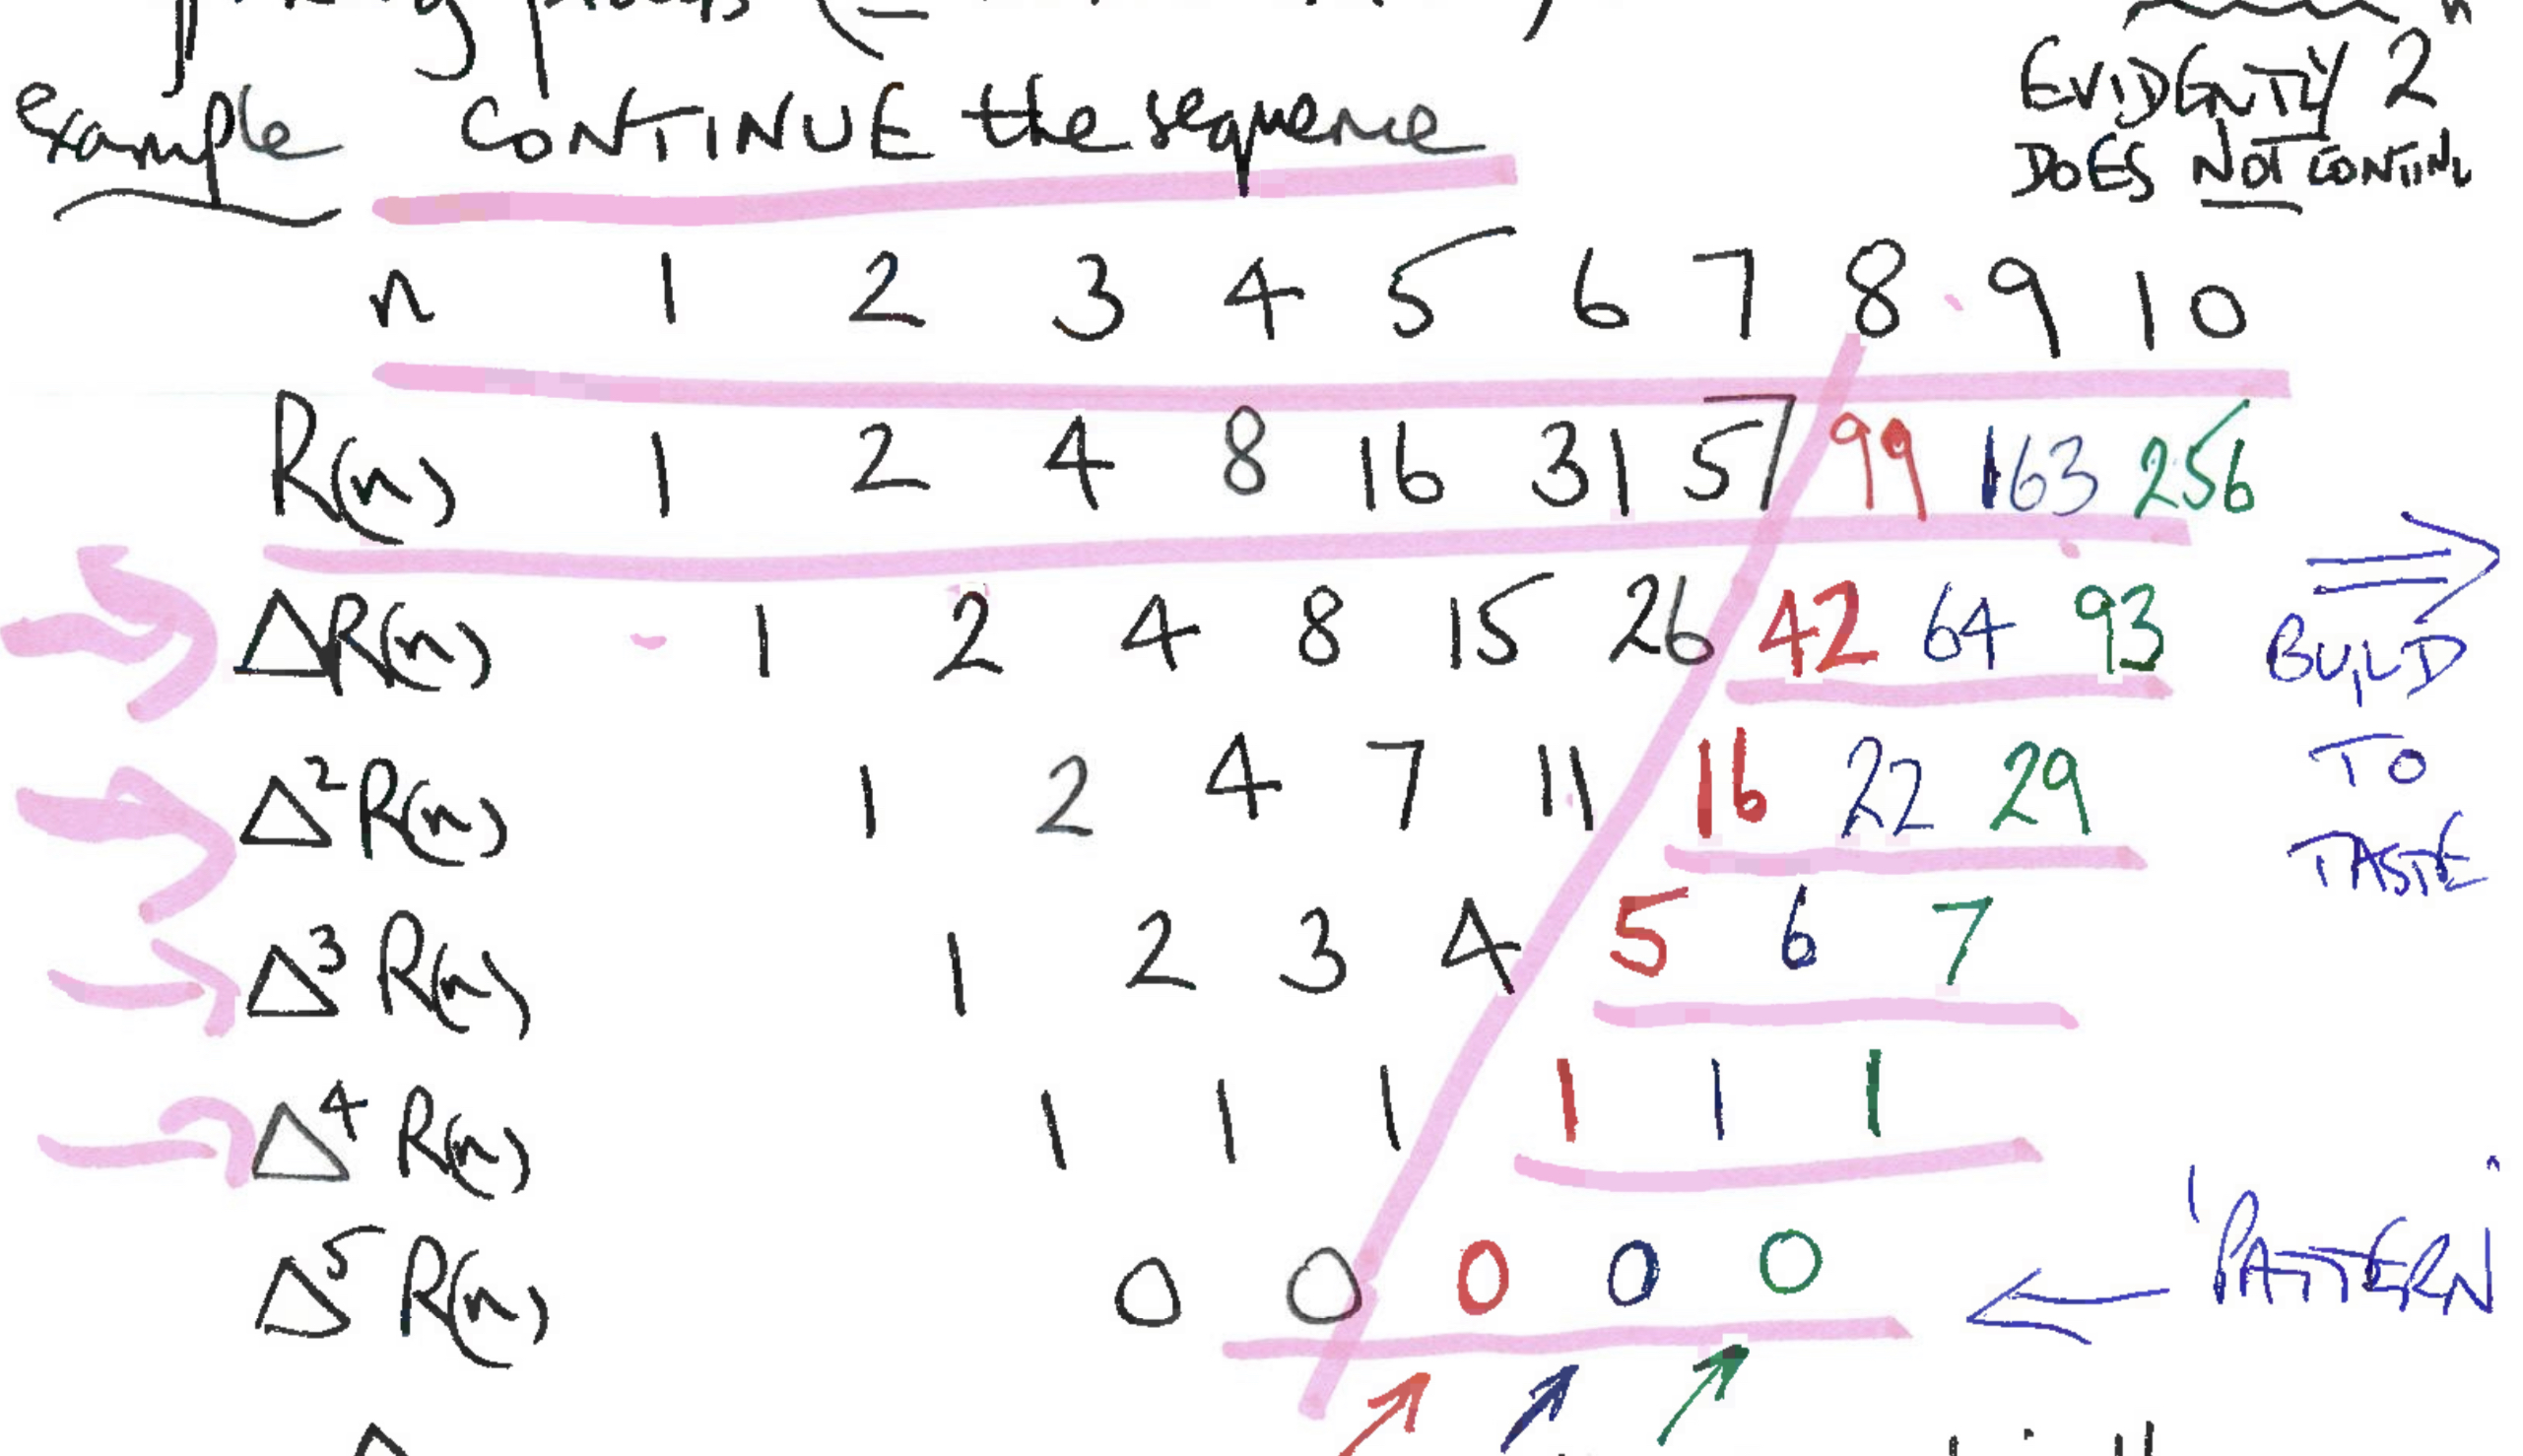
\includegraphics[scale = 0.15]{inverseDifferencing.jpg}
    \centering
    \caption{graph of reverse differencing porcess}\label{fig:invDiff}
    % In figure env, label is always after caption for it to function normally.
    \end{figure}
    
    \noindent And and example of the \emph{inverse} process is as shown in figure~\ref{fig:invDiff}.
    To find out the sequence of $R(n)$ beyond $n = 7$, one can keep on differencing
    the sequence (which is \emph{polynomial-like}) until its fourth and fifth order,
    realizing the repetitive $0$s and $1$s pattern, construct further 1s and 0s,
    and do the inverse back until order 0, i.e.\ constructing $R(n)$. 
    The pattern continues, in fact, only when $R(n)$ is a $k = 4$ degree polynomial in $n$.

    \medskip
    \noindent \underline{Note}: (Not in syllabus) There is a discrete analogy to Taylor's expansion,
    involving Newton's forward difference interpolation formula \ldots
\end{ex}

The sequence in the inverse process is actually\[
    \begin{align*} 
        & \begin{aligned}
        1 + (n - 1) + \frac{1}{2}(n-1)(n-2) & + \frac{1}{6}(n-1)(n-2)(n-3) \\
                                            & + \frac{1}{24}(n-1)(n-2)(n-3)(n-4) 
        \end{aligned} \\
                    & = \begin{pmatrix}
                            n-1 \\
                            0
                    \end{pmatrix} + \begin{pmatrix}
                            n-1 \\
                            1
                    \end{pmatrix} + \begin{pmatrix}
                            n-1 \\
                            2
                    \end{pmatrix} + \begin{pmatrix}
                            n-1 \\
                            3
                    \end{pmatrix} + \begin{pmatrix}
                            n-1 \\
                            4
                    \end{pmatrix} \\
                    & = \begin{pmatrix}
                            n \\
                            0
                    \end{pmatrix} + \begin{pmatrix}
                            n \\
                            2
                    \end{pmatrix} + \begin{pmatrix}
                            n \\
                            4
                    \end{pmatrix}.
    \end{align*}
\]
\begin{figure}
  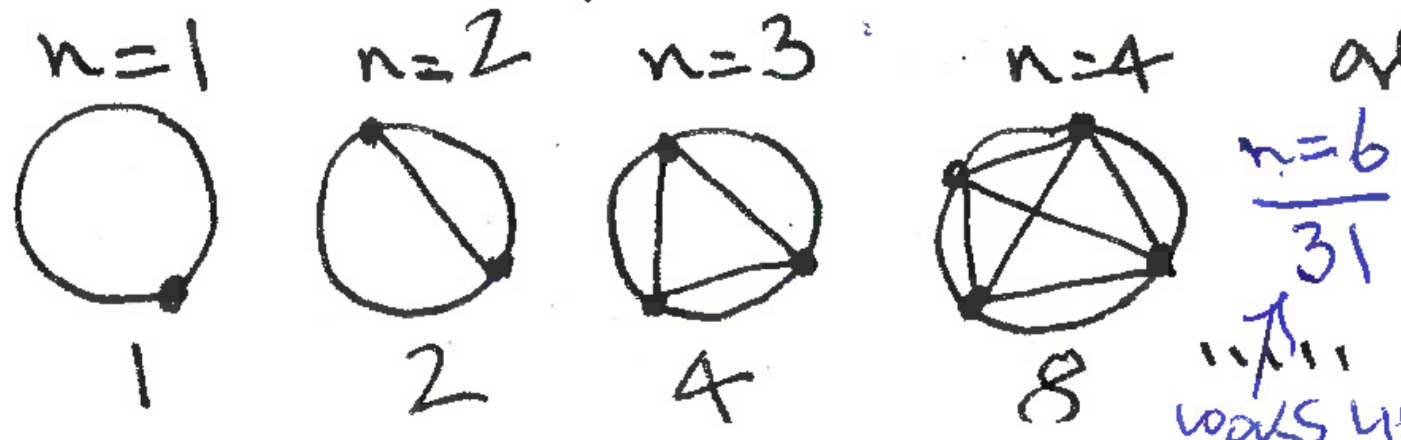
\includegraphics[scale=0.15]{circlePartition.jpeg}
  \centering
  \caption{Circle Division}\label{fig:circDiv}
\end{figure}

This expression represents the numbers of distinct regions into which the interior of a circle
is partitioned when $n$ distinct boundary points are connected by straight lines, as shown in figure~\ref{fig:circDiv}.
This is, however, not easy to prove!


\subsection{First Order Recurrence/Discrete Nonlinear Systems}

Consider $x_{n + 1} = F(x_n)$ where $x_n = x(n), x_n \neq 0$.
And we have initial choice $x_0$: \[
    \Rightarrow{} x_1 = F(x_0)
    \Rightarrow{} x_2 = F(x_1) = F(F(x_0)) = F^{(2)}(x_0) \Rightarrow{} \ldots
\]

This process is called \textbf{\emph{iteration}} ---
some function is used repeatedly --- \emph{iterative process}.
We can repersent this process graphically, as shown in Figure~\ref{fig:cobweb}.

\begin{figure}
  	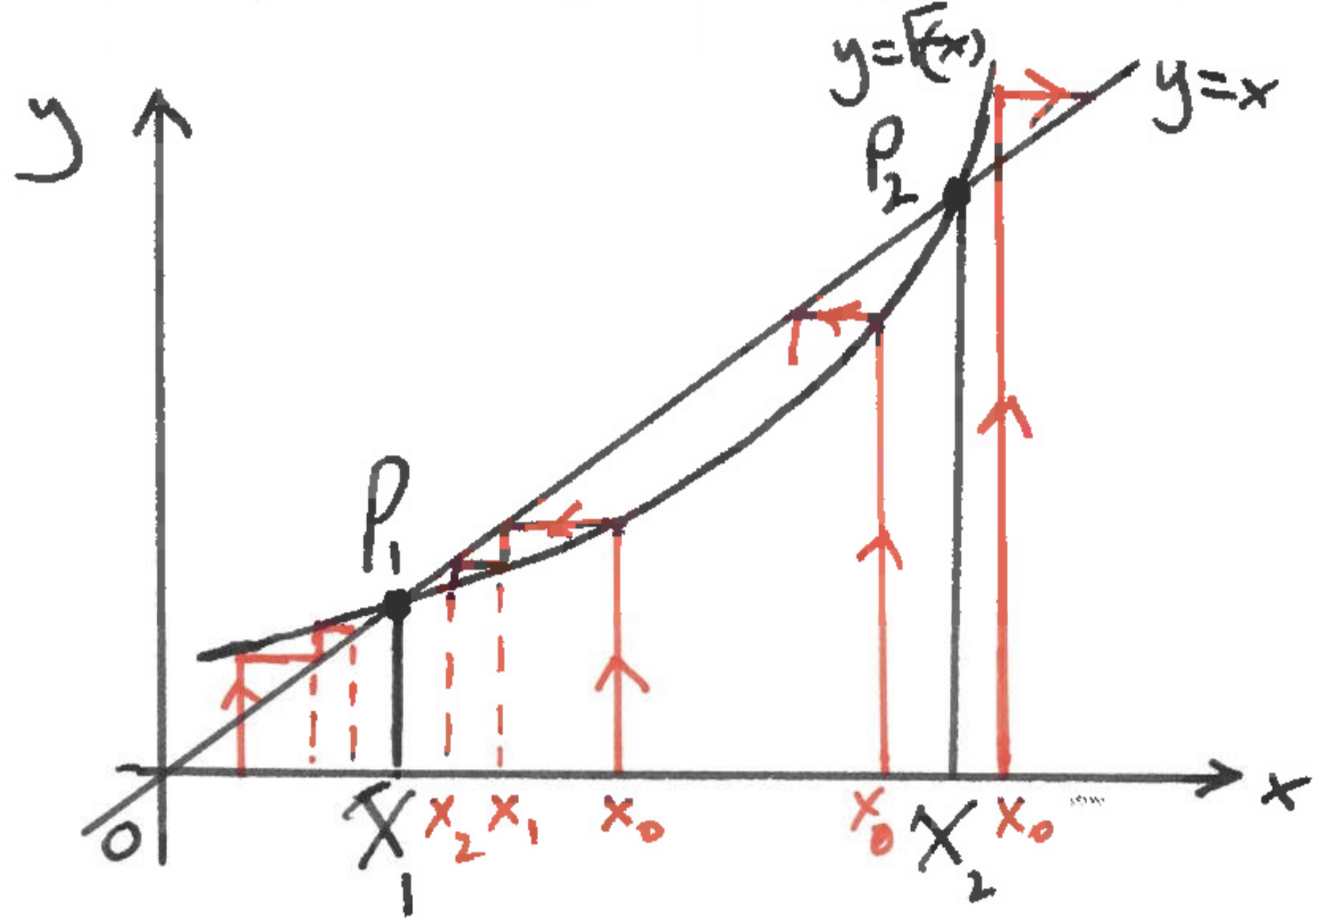
\includegraphics[scale=0.15]{CobwebDiagram.jpg}
  	\centering
    \caption{'Cobweb' Diagram}\label{fig:cobweb}
\end{figure}

There are 2 fixed points $P_1$ and $P_2$, for which the $x$ values satisfy\[
    X = F(X) \Rightarrow{} X_1, X_2.
\]
However, the \emph{character} of $P_1$ and $P_2$ is very different ---
initial values $x_0$ which start near $X_1$ have $x_n$ which approaches $X_1$,
while those $x_0$ which start near $X_2$ certainly are \emph{not} giving $x_n$
which approaches $X_2$!

\newmdtheoremenv[style=defEnv]{attractor and repeller}[theorem]{Definition}
\begin{attractor and repeller}
    $X_1$ corresponding to $P_1$ is said to be \textbf{\emph{asymptotically stable}} or \emph{attracting},
    and is called \textbf{\emph{attractor}};
    $X_2$ corresponding to $P_2$ is said to be \textbf{\emph{unstable}} or \emph{repelling},
    and is called \textbf{\emph{repeller}}.
\end{attractor and repeller}

How can we distinguish them analytically?

\medskip
Suppose $x_{n + 1} = F(x_n)$ and $X = F(X)$.
We put $X = x_n + \epsilon_n$ and imagine $x_0$ is chosen so that
$\epsilon_0$ is `small' i.e.\ $x_0$ is `near' to $X$.
Let's see how $\epsilon_n$ develops (whether $x_n$ converges or diverges to $X$):\[
        X - \epsilon_{n + 1} & = x_{n + 1} = F(x_n) = F(X - \epsilon_n)
        = F(X) - \epsilon_n F'(X) + \frac{1}{2}\epsilon_n^{2}F(X) + \cdots
        \]with the last step using taylor expansion, and by cancelling $X$ and $F(X)$, we get\[
        \epsilon_{n + 1} = \epsilon_n F'(X) - \frac{1}{2}\epsilon_n^{2}F''(X) + \cdots.
\]
$\epsilon_{n + 1}$ can therefore be estimated using different values of the various orders of $F(X)$:
\begin{itemize}
    \item $F'(X) \neq 0 \Rightarrow{} \epsilon_{n+1} \approx \epsilon_n F'(X)
        \Rightarrow{} \epsilon_n \approx \epsilon_0 {[F'(X)]}^{n}$.

        This process is called \textbf{\underline{first order process}}.
        Then if $|F'(X)|<1$, then $\epsilon_n \rightarrow{} 0$ and $X$ is an attractor.
        Otherwise if $|F'(X)|>1$, then $\epsilon_n$ diverges and $X$ is a repeller.
        However, if $|F'(X)| = 1$ then it depends on the case --- nothing is already proven.

    \item $F'(X) = 0, F''(X) \neq 0 \Rightarrow{} \epsilon \approx -\frac{1}{2}\epsilon_n^{2}F''(X)
        \Rightarrow{} \epsilon_{n + 1} \propto \epsilon_n^{2}$.

        This process is called \textbf{\underline{second order process}}.
        $\forall \epsilon_0$ sufficiently small, we have $\epsilon_n \rightarrow{} 0$,
        and $X$ is \emph{always} an attractor. 
        (Proof is not provided here.)
        
        Note that it is \emph{faster} than first order convergence,
        therefore it is usually preferred to design a process such that it is
        second order for studying that particular matter for better result.

    \item $F'(X) = 0, F''(X) = 0, F'''(X) \neq 0 \Rightarrow{} \epsilon_{n + 1} \propto \epsilon_n^{3}$.%chktex 23

        This process is called \textbf{\underline{third order process}}.
\end{itemize}
And so on. The \emph{rate} of convergence increases with the order of the process.
Third order process and beyond are usually unnecessary, but occasionally they
may be required. In practice we hope for second order,
but will often settle for first order.

\begin{ex}
    \,

    \begin{enumerate}[label = (\alph*)]
        \item \[
                x_{n+1} = \frac{1}{2}\left(x_n + \frac{A}{x_n}\right) = F(x_n)
        \]
        which is a method for finding $\sqrt{A}$.
        For instance, $A=12, x_0 = 2, \ldots, x_4 = 3.4641$, etc.

        The fixed points are $X = \frac{1}{2}\left(X + \frac{A}{X}\right)
        \rightarrow{} X = \pm \sqrt{A}$. By drawing the Cobweb diagram, we should see that
        $x_0 > 0 \Rightarrow{} x_n \rightarrow{} \sqrt{A}, x_0 < 0 \Rightarrow{} x_n \rightarrow{} \sqrt{A}$.

        Next we find out which order the process is:\[
            \begin{align*}
                F'(X)  & = \frac{1}{2}\left(1 - \frac{A}{X^{2}}\right) = 0 \\
                F''(X) & = \frac{A}{X^{3}} = \pm \frac{1}{\sqrt{A}} \neq 0.
            \end{align*}
        \]
        So this is a second order process, and $\pm \sqrt{A}$ are attractors with
        $\epsilon_{n + 1} \propto \epsilon_{n}^{2}$.

        \underline{Exercise}: Consider $A < 0$?

    \item Solve\[
            f(x) = x^{2} - 6x + 2 = 0.
    \]
    We can rearrange this in various ways and write it in iterative process:
    \begin{enumerate}[label = (\roman*)]
        \item $x_{n + 1} = 6 - \frac{2}{x}$
        \item $x_{n + 1} = \frac{1}{6}x_n^{2} + \frac{1}{3}$
        \item $x_{n + 1} = \sqrt{6x_n - 2}$
        \item $x_{n + 1} = x_n - \frac{x_n^{2} - 6x_n + 2}{2x - 6}
            = \frac{x_n^{2} - 2}{2x_n - 6}$.
    \end{enumerate}

    Examining these (see Problem Sheet 3) we find that (iv) is the `best buy'
    in that it is the \emph{only} second order process and it is the only one
    which allows us to obtain both roots and attractors if we choose $x_0$ suitably.

\item \[
        x_{n + 1} = x_n (2 - Ax_n)
\]
which is a method for finding a reciprocal \emph{without} division! ($x_n \rightarrow{} \frac{1}{A}$)
It is a second order process.

\underline{Note}: Examples (a), (b)(iv), (c) are examples of what is now called %chktex 36
the \emph{Newton(-Raphson) Method} for finding solutions of $f(x) = 0$: \[%chktex 36
    x_{n + 1} = F(x_n) = x_n - \frac{f(x_n)}{f'(x_n)}.
\]
Such a process is \emph{normally} at least second order (good!) because \[
    F'(x) = 1 - \frac{f'(x)}{f'(x)} + \frac{f(x)f''(x)}{{(f'(x))}^{2}} = 0
\]and\[
F''(x) = \frac{f''(x)}{f'(x)} \neq 0 \;\textnormal{usually}.
\]
However, there are some difficulties in implementing the method successfully,
including choosing a value near roots, having multiple roots, etc.
    
\item modern, practical, surprising\ldots \underline{Population Dynamics}

    Recall the \emph{logistic map equation}:\[
        P(n + 1) = aP(n) - b{(P(n))}^{2}
    \]
    which is a simple mathematical model with very complicated dynammics.
    Put $x_n = \frac{b}{a}P(n)$, and we get\[
        x_{n + 1} = ax_n(1 - x_n)
    \]
    with $a$ being the constant. This is the standard form of logistic map.

    Although there is no restriction for mathematical interest,
    the `physical' interest is in $0 \le a \le 4$ so that $[0, 1] \rightarrow{} [0, 1]$.
    We can easily see that the maximum value that $x_n (1 - x_n)$ can get is $\frac{1}{4}$,
    therefore having any $a > 4$ would definitely result in $x_{n + 1} > 1 \Rightarrow{}
    x_{n + 2} < 0$, and let alone $a < 0$.
    We certainly would not want negative population values!

    There are evidently two fixed points satisfying\[
        X = aX(1 - X) \Rightarrow{} X = 0 \;\textnormal{and}\; X = 1 - \frac{1}{a}.
    \]
    Which do we get, and when?
    Take the first order process and analyse with different ranges of $a$:\[
        |F'(X)| = |a(1 - 2X)|.
    \]
    \begin{itemize}
        \item $0 \le a < 1$, $a = 0$ is trivial.

            We can deduce that $x = 0$ is an attractor,
            while $x = 1 - \frac{1}{a}$ is a repeller.
            This makes sense because it is a linear model made worse by overcrowding.

        \item $1 < a < 3$.

            We can decude that $x= 0$ is a repeller,
            while $x = 1 - \frac{1}{a}$ is an attractor.
            This makes sense because it is an exponential growth stabilised by overcrowding.

            This behaviour is very similar to that of the logistic differential equation
            --- what follows is definitely not so!

        \item $a > 3$.

            We can deduce that $x = 0$ and $x = 1 - \frac{1}{a}$ are both repellers.

            So what exactly do we get?
            We get `\emph{period doubling}'.

            \medskip
            Consider $x_{n + 2} = F(x_{n + 1}) = F(F(x_{n})) = F^{(2)}(x_n)
            = a[ax_n (1 - x_n)][1 - ax_n(1 - x_n)]$.
            The fixed points of this satisfy
            \begin{equation}\label{eqn:1}
                X = a^{2}X(1 - X)[1 - aX(1-X)]
            \end{equation}
            We still have $X = 0, X = 1 - \frac{1}{a}$ of course,
            but now we have two new ones, say $X_1$ and $X_2$, satisfying
            \begin{equation}\label{eqn:2}
                a^{2}X^{2} - a(a+1)X + (a+1) = 0
            \end{equation}
            which is derived from dividing equation~\eqref{eqn:1} with the two known solutions.
            (Or do factorization accordingly.) We also know that $X_1 = F(F(X_1)), X_2 = F(F(X_2))$,
            and thus we must have\[
                X_1 = F(X_2), \quad X_2 = F(X_1)
            \]
            because with $F(X_1) = F(F(F(X_1)))$, $F(X_1)$ being the solution to itself 
            being applied to $F$ twice, there is nothing other than $X_2$ 
            which can possibly be the value of $F(X_1)$: The two known values cannot be duplicated,
            and $X_1$ itself is a repeller, thereby impossible to be a fixed point of the map.
            Similarly for the value of $X_1$, $X_1 = F(X_2)$.

            This forms a \emph{flip} or \emph{2-cycle}. (Before becoming 4-cycle, 8-cycle, etc.)
            This is an attractor when\[
                \left|\frac{\mathrm{d}}{\mathrm{d}x} F(F(x)) \right| < 1
            \]\[
                \Rightarrow{} |F'(X_1)F'(X_2)| < 1,
                |a(1 - 2X_1) a(1 - 2X_2)| < 1
            \]and using Vieta's theorem to obtain the sum and product of the two roots
            from equation~\eqref{eqn:2}, we get\[
                3 < a < 1 + \sqrt{6}
            \]
            for positive $a$. For increasingly larger $a > 1 + \sqrt{6}$, we then obtain 4 cycle
            $\Rightarrow{}$ 8 cycle $\Rightarrow{} \ldots \Rightarrow{}$ $2^{\infty}$ cycle.
    \end{itemize}
    \end{enumerate}
    
\end{ex}

\paragraph{Novelty!}
The stable windows get shorter in geometrical progression
at rate $\frac{1}{4.669\ldots}$, where $4.669\ldots$ is the \emph{\underline{Feigenbaum constant}}.
(The first one. There is another one, which is not introduced by Berkshire.)
For $3.57 < a \le 4$, `Chaos' + periodic windows!


\section{Linear Systems of Differential Equations}





\chapter{Linear Algebra}

\section{Introduction to Matrices and Vectors}

\subsection{Column vectors}

\newmdtheoremenv[style=defEnv]{column vector}[theorem]{Definition}
\begin{column vector}
    A \emph{column vector} ($n$-column vector) $\pmb{v}_n$ is a tuple of $n$ real numbers written as a single columnn, 
    with $a_1, a_2, a_3, \ldots, a_n \in \mathbb{R}$:\[
    \pmb{v}_n := 
    \begin{pmatrix}
        a_1 \\
        a_2 \\
        a_3 \\
        \vdots \\
        a_n
    \end{pmatrix}
    \]
\end{column vector}

\newmdtheoremenv[style=defEnv]{set of column vectors}[theorem]{Definition}
\begin{set of column vectors}
    $\mathbb{R}^{n}$ is the set of all column vectors of height $n$ whose entries are real numbers.
    In symbols:\[
        \mathbb{R}^{n} = \{
            \begin{pmatrix}
                    a_1\\
                    a_2\\
                    \vdots\\
                    a_n
            \end{pmatrix}
            : a_1, a_2, \ldots, a_n \in \mathbb{R}
        \} 
    \]
\end{set of column vectors}

\begin{ex}
    $\mathbb{R}^{2}$ can be seen as Euclidean plane. $\mathbb{R}^{3}$ can be seen as Euclidean space.
    \\\underline{Caution}: Our vectors always ``start'' at the origin.
\end{ex}

\newmdtheoremenv[style=defEnv]{zero vector}[theorem]{Definition}
\begin{zero vector}
    The \textbf{\emph{zero vector $\pmb{0}_n$}} is the height $n$-column vector all of whose entries are 0.
\end{zero vector}


\newmdtheoremenv[style=defEnv]{standard basis vector}[theorem]{Definition}
\begin{standard basis vector}
    The \textbf{\emph{standard basis vectors}} in $\mathbb{R}^{n}$ are the vectors\[
        \pmb{e}_1 = \begin{pmatrix}
                1\\
                0\\
                \vdots\\
                0
        \end{pmatrix}, \quad
        \pmb{e}_2 = \begin{pmatrix}
                0\\
                1\\
                \vdots\\
                0
        \end{pmatrix}, \quad \ldots, \quad
        \pmb{e}_n = \begin{pmatrix}
                0\\
                0\\
                \vdots\\
                1
        \end{pmatrix}
    \]
    i.e. $\pmb{e}_k$ is the vector with $k$th entry equal to 1 and all other entries equal to 0.
\end{standard basis vector}

\paragraph{Operations on column vectors}

    \[
        \pmb{v} := \begin{pmatrix}
                v_1\\
                v_2\\
                \vdots\\
                v_n
        \end{pmatrix}, \quad
        \pmb{u} := \begin{pmatrix}
                u_1\\
                u_2\\
                \vdots\\
                u_n
            \end{pmatrix}
    \]
    be column vectors $\mathbb{R}^{n}$, and let $\lambda$ be a (real or complex) number.
    \begin{enumerate}[label = (\arabic*)]
        \item Addition on vectors in $\mathbb{R}^{n}$ is given by:\[
                \begin{pmatrix}
                        v_1 + u_1\\
                        v_2 + u_2\\
                        \vdots\\
                        v_n + u_n
                \end{pmatrix}
            \]$+ : \mathbb{R}^{n} \times \mathbb{R}^{n} \rightarrow \mathbb{R}^{n}$ (binary operatioin).
            $(\mathbb{R}^{n}, +)$ is a group.
        \item \textbf{\emph{Scalar multiplication}} $\lambda \pmb{v}$ on $\mathbb{R}^{n}$:\[
            \begin{pmatrix}
                    \lambda v_1\\
                    \lambda v_2\\
                    \vdots\\
                    \lambda v_n
            \end{pmatrix}
        \]$s : \mathbb{R} \times \mathbb{R}^{n} \rightarrow \mathbb{R}^{n}$, so not binary operation.
    \item \textbf{\emph{Dot product}} $v \cdot u$ is defined to be the number $v_1 u_1 + v_2 u_2 + \cdots + v_n u_n$.
            $\cdot : \mathbb{R}^{n} \times \mathbb{R}^{n} \rightarrow \mathbb{R}$, so not binary.
    \end{enumerate}

\begin{ex}
    Show that $(\mathbb{R}^{n}, +)$ is an Abelian group.
    \begin{itemize}
        \item Identity: $\pmb{0}_n$ ($v + \pmb{0}_n = \pmb{v}$)
        \item $-\pmb{v}$ are inverses, where \[
            -\pmb{v} := \begin{pmatrix}
                    -v_1\\
                    -v_2\\
                    \vdots\\
                    -v_n
            \end{pmatrix}
        \]
        \item associativity: $(\pmb{u} + \pmb{v}) + \pmb{w} = \pmb{u} + (\pmb{v} + \pmb{w})$.
        \item commutative: $\pmb{u} + \pmb{v} = \pmb{v} + \pmb{u}$
    \end{itemize}
    \underline{Caution}: $+$ only makes sense for vectors of the \emph{same size}.
    e.g. $\pmb{v} \cdot \pmb{0}_n = 0 \in \mathbb{R}$.
\end{ex}

\newmdtheoremenv[style=defEnv]{combination of add and scalar multi}[theorem]{Definition}
\begin{combination of add and scalar multi}
    let $\pmb{v}_1, \pmb{v}_2, \pmb{v}_3, \ldots, \pmb{v}_n \in \mathbb{R}^{n}, \lambda_1, \lambda_2, \lambda_3, \ldots, \lambda_n \in \mathbb{R}$,
    then \[
        \lambda_1 \pmb{v}_1 + \lambda_2 \pmb{v}_2 + \cdots + \lambda_n \pmb{v}_n
    \]is called a \textbf{\emph{linear combination}} of $\pmb{v}_1, \pmb{v}_2, \pmb{v}_3, \ldots, \pmb{v}_n$.
\end{combination of add and scalar multi}

\newmdtheoremenv[style=defEnv]{span of vectors}[theorem]{Definition}
\begin{span of vectors}
    The set of all linear combinatioins of a collection of vectors $\pmb{v}_1, \pmb{v}_2, \ldots, \pmb{v}_n$
    is called the \textbf{\emph{span}} of the vectors $\pmb{v}_1, \pmb{v}_2, \ldots, \pmb{v}_n$.
    \\Notation: 
    
    span$\left\{\pmb{v}_1, \pmb{v}_2,\ldots,\pmb{v}_n\right\} := 
    \left\{\lambda_1 \pmb{v}_1 + \lambda_2 \pmb{v}_2 + \cdots + \lambda_n \pmb{v}_n 
    | \lambda_1, \ldots, \lambda_n \in \mathbb{R}\right\}$
\end{span of vectors}

\begin{ex}
    compute the span of 
    \begin{itemize}
        \item $\{\pmb{e}_1, \pmb{e}_2\}$, $\pmb{e}_1, \pmb{e}_2 \in \mathbb{R}^2$.
            \[
                \textnormal{span}\{\pmb{e}_1, \pmb{e}_2\} 
                = \{\lambda_1 \pmb{e}_1 + \lambda_2 \pmb{e}_2 | \lambda_1, \lambda_2 \in \mathbb{R}\}
            = \{
                    \begin{pmatrix}
                            \lambda_1\\
                            \lambda_2
                    \end{pmatrix}
| \lambda_1, \lambda_2 \in\mathbb{R}\}\]

\item span$\left\{\begin{pmatrix}
        1\\
        0\\
        0
\end{pmatrix}
, \begin{pmatrix}
        0\\
        2\\
        0
\end{pmatrix}
\right\} = \{
\begin{pmatrix}
        \lambda_1\\
        2\lambda_2\\
        0
\end{pmatrix}
| \lambda_1, \lambda_2 \in \mathbb{R}
\}$
    \end{itemize}
    
\end{ex}

\newmdtheoremenv[style=defEnv]{length and norm}[theorem]{Definition}
\begin{length and norm}
    let $\pmb{v} \in \mathbb{R}^{n}$. The \textbf{\emph{length}} of $\pmb{v}$, a.k.a.\ the \textbf{\emph{norm}} 
    of $\pmb{v}$, is the non-negative real number $\lVert\pmb{v}\rVert$ defined by \[
        \lVert\pmb{v}\rVert = \sqrt{\pmb{v} \cdot \pmb{v}}
    \]
    \underline{Note}: $\lVert\pmb{0}\rVert = 0$, and conversely if $\pmb{v} \neq 0$ then $\lVert\pmb{v}\rVert > 0$.
    This definition agrees with out usual ideas about the length of a vector in $\mathbb{R}^{2}$
    or $\mathbb{R}^{3}$, which follows from Pythagoras' theorem.
\end{length and norm}

\newmdtheoremenv[style=defEnv]{unit vector}[theorem]{Definition}
\begin{unit vector}
    A vector $\pmb{v} \in \mathbb{R}^{n}$ is called a \textbf{\emph{unit vector}}
    if $\lVert\pmb{v}\rVert = 1$.
\end{unit vector}

\smallskip
\begin{ex}
    \;

    \begin{enumerate}[label = (\arabic*)]
        \item Any non-zero vector $\pmb{v}$ can be made into a unit vector
            $\hat{\pmb{u}} := \frac{\pmb{v}}{\lVert\pmb{v}\rVert}$. This process is called \textbf{\emph{normalizing}}.
        \item The standard basis vectors are unit vectors.
    \end{enumerate}
    
\end{ex}

\subsection{Basic Matrix Operations}

\newmdtheoremenv[style=defEnv]{matrix definition}[theorem]{Definition}
\begin{matrix definition}
    An $n \times m$-matrix is a rectangular grid of numbers called the \emph{entries} of the matrix
    with $n$ rows and $m$ columns. A real matrix is onne whose entries are real numbers,
    and a complex matrix is one whose entries are complex numbers.

    \underline{Notations}: $M_{n \times m}(\mathbb{R}), M_{n,m}(\mathbb{R}), \mbox{Mat}_{n\times m}(\mathbb{R}), \mathbb{R}^{n\times m}$.

\end{matrix definition}

\underline{Operations on matrices}:
\newmdtheoremenv[style=defEnv]{matrices operation}[theorem]{Definition}
\begin{matrices operation}
    let $A = (a_{ij})$ and $B = (b_{ij})$ are $n\times m$-matrix, $\lambda \in \mathbb{R}$. Then:
    \begin{enumerate}[label = (\arabic*)]
        \item $A+B = n\times m$-matrix $\,(a_{ij} + b_{ij})$.
            $+: M_{n \times m}(\mathbb{R}) \times M_{n \times m}(\mathbb{R}) \rightarrow M_{n \times m}(\mathbb{R})$
        \item $\lambda A = n \times m$-matrix $\,(\lambda a_{ij})$
    \end{enumerate}
    
\end{matrices operation}

\newmdtheoremenv[style=defEnv]{addition on matrix is Abelian}[theorem]{Theorem}
\begin{addition on matrix is Abelian}
    $(M_{n \times m}(\mathbb{R}), +)$ is an Abelian grouop.
\end{addition on matrix is Abelian}

\newmdtheoremenv[style=defEnv]{transpose}[theorem]{Definition}
\begin{transpose}
    The \textbf{\emph{transpose}} $A^{T}$ of an $n \times m$-matrix $(a_{ij})$ is 
    the $m \times n$-matrix $(a_{ij})$.
    The \textbf{\emph{leading diagonal}} of a matrix is the $(1, 1), (2, 2), \ldots$ entries.
    So the transpose is obtained by doing a reflection in the leading diagonal.
\end{transpose}

\newmdtheoremenv[style=defEnv]{multiplying matrix with vector}[theorem]{(Multiplying matrices with vectors) Definition}
\begin{multiplying matrix with vector}
    Let $A = (a_{ij})$ be an $n \times m$-matrix, $\pmb{v} \in \mathbb{R}^{m}$.
    Then $A\pmb{v}$ is the vector in $\mathbb{R}^{n}$ with $i$-th row entry $\sum_{j=1}^{m} a_{ij}\pmb{v}_j$
\end{multiplying matrix with vector}

\begin{ex}
    \;

    \begin{itemize}
            \item 
                Prove that for $A \in M_{n \times m}(\mathbb{R}), \pmb{e}_k \in \mathbb{R}^{m}$,
                $A\pmb{e}_k = k$-th column of A.
    
                \underline{Proof}: let $A = (a_{ij})$. By definition the $i$-th entry of $A\pmb{e}_k$ is\[
                    \sum_{j=1}^{m} a_{ij}{(\pmb{e}_k)}_j = a_{ik}
                \]since $ {(\pmb{e}_k)}_j = 0$ whenever $j \neq k$, 1 for $j = k$
            \item Let $I_n$ be the identity matrix. Show formally that $I_n \pmb{\nu} = \pmb{\nu}$, $\forall \pmb{\nu} \in \mathbb{R}^{n}$.
            \item $\pmb{\nu} \cdot \pmb{v} = \pmb{\nu}^{T} \pmb{v}$
            \item let $\pmb{\nu}_1, \pmb{\nu}_2, \pmb{\nu}_3 \in \mathbb{R}^{3}$.
                Write the linear combination $3\pmb{\nu}_1 - 5\pmb{\nu}_2 + 7\pmb{\nu}_3$ as a multiplication of matrix
                $A \in M_{3 \times 3}(\mathbb{R})$ with a vector $\pmb{x} \in \mathbb{R}^{3}$. Then\[
                    A\pmb{x} = \begin{pmatrix}
                        \pmb{\nu}_1 & \pmb{\nu}_2 & \pmb{\nu}_3
                    \end{pmatrix} 
                    \begin{pmatrix}
                            x_1 \\
                            x_2 \\
                            x_3
                    \end{pmatrix} 
                    = x_1\pmb{\nu}_1 + x_2\pmb{\nu}_2 + x_3\pmb{\nu}_3
                \]
                with $\pmb{\nu}_1, \pmb{\nu}_2, \pmb{\nu}_3$ written as a column vector to form a matrix
                in the above expression, thus using matrix multiplication to express linear combination of vectors.
    \end{itemize}
    
\end{ex}

\section{Systems of linear equations}

\subsection{Definitions}

\newmdtheoremenv[style=defEnv]{linear equation}[theorem]{Definition}
\begin{linear equation}
    A \textbf{\emph{linear equation}} in the variables $x_1, x_2, \ldots, x_n \in \mathbb{R}$
    is an equation of the form:\[
        \lambda_1 x_1 + \lambda_2 x_2 + \cdots + \lambda_n x_n = c, 
        \,\textnormal{with }\, \lambda_1,\ldots,\lambda_n \subset \,\textnormal{\emph{Fixed} real numbers}
    \]
    \underline{Caution}: In particular, no powers/multiplications/function of one or more variables.
\end{linear equation}

\newmdtheoremenv[style=defEnv]{simultaneous list of linear equations}[theorem]{Definition}
\begin{simultaneous list of linear equations}
    A system of $n$ linear equations is a list of simultaneous linear equations.
    It can be converted to $A\pmb{x} = \pmb{b} \in \mathbb{R}^{m}$,with\[
        A = \begin{pmatrix}
            a_{11} & a_{12} & \cdots & a_{1n} \\
            a_{21} & a_{22} & \cdots & a_{2n} \\
            \vdots & \vdots & \ddots & \vdots \\
            a_{m1} & a_{m2} & \cdots & a_{mn}
        \end{pmatrix} 
        \in \mathbb{R}^{m \times n}
    \]
\end{simultaneous list of linear equations}
\underline{Caution}: Thee $m \times n$-matrix $A$ is called coefficient matrix.
The matrix $(A|\pmb{b})$ where the vector $\pmb{b}$ is added as a column on the  right
is called \textbf{\emph{augmented matrix}}.

\newmdtheoremenv[style=defEnv]{consistent system}[theorem]{Definition}
\begin{consistent system}
    A system is called \textbf{\emph{consistent}} (resp.\ inconsistent)
    if it has a solution $(s_1, s_2, \ldots, s_m)$ (resp.\ no solution).
\end{consistent system}

\begin{ex}
    \[\left\{
        \begin{align*}
            & x_1 + x_3 - x_4 = 1 \\
            & x_2 - x_4 = 6 \\
            & x_1 + x_2 + 6x_3 - 3x_4 = 0
        \end{align*}
     \right.   
    \]
    Augmented matrix form:\[
        \left(\begin{array}{@{}cccc|c@{}}%chktex 4, chktex 44
                1 & 0 & 1 & -1 & 1 \\
                0 & 1 & 0 & -1 & 6 \\
                1 & 1 & 6 & -3 & 0
        \end{array}\right)
    \]
\end{ex}

\newmdtheoremenv[style=defEnv]{row operation}[theorem]{Definition}
\begin{row operation}
    A \textbf{\emph{row operation}} is one of the following procedures on a $n \times m$-matrix $(a_{ij})$:
    \begin{enumerate}[label = (\arabic*)]
        \item $r_i(\lambda)$: multiply row $i$ by a scalar $\lambda \in \mathbb{R}, \lambda \neq 0$.
        \item $r_{ij}$: swap row $i$ with row $j$.
        \item $r_{ij}(\lambda)$: multiply row $i$ by $\lambda \neq 0$, $\lambda \in \mathbb{R}$ and add it to row $j$.
    \end{enumerate}
\end{row operation}

\begin{ex}
    let $A = \begin{pmatrix}
        1 & 2 \\
        3 & 4
    \end{pmatrix} $, so\[
        r_{12} \Rightarrow \begin{pmatrix}
            3 & 4 \\ 
            1 & 2
        \end{pmatrix} 
    \]\[
    r_2(2) \Rightarrow \begin{pmatrix}
        1 & 2\\
        6 & 8
    \end{pmatrix} 
    \]\[
    r_{12}(2) \Rightarrow \begin{pmatrix}
        1 & 2 \\
        5 & 8
    \end{pmatrix} 
    \]
\end{ex}

\newmdtheoremenv[style=defEnv]{row operation on augmented matrix}[theorem]{Proposition}
\begin{row operation on augmented matrix}
    Let $A\pmb{x} = \pmb{b}$ be a system of linear equations in matrix form, $(A|\pmb{b})$
    the augmented matrix, $(A'|\pmb{b}')$ the augmented matrix of the system after row operation.
    Show that $x$ is solution of $A\pmb{x} = \pmb{b} \iff$ $x$ is solution of $A'\pmb{x} = \pmb{b}'$.
\end{row operation on augmented matrix}

\begin{proof}
    row operations of type (1) and (2) $\Rightarrow$ trivial.%chktex 10

    (3) Take equation $i$, multiply it by $\lambda$, add it to equation $j$.
    $\Rightarrow (a_{j1} + \lambda a_{i 1}) x_1 + \cdots + (a_{jm} + \lambda a_{im})x_m = b_j + \lambda b_i$.
\end{proof}
\underline{Caution}: Every row operation is invertible: \[
    {[r_i(\lambda)]}^{-1} = r_i(\frac{1}{\lambda}),\; {[r_{ij}]}^{-1} = r_{ij},\;
    {[r_{ij}(\lambda)]}^{-1} = r_{ij}(-\lambda)
\]

\subsection{Gauss algorithm}
\newmdtheoremenv[style=defEnv]{echelon form}[theorem]{Definition}
\begin{echelon form}
    The left most non-zero entry in a non-zero row is called \textbf{\emph{leading entry}}.
    A matrix is called in \textbf{\emph{echelon form}} if:
    \begin{enumerate}[label = (\arabic*)]
        \item The leading entry in each non-zero row is 1.
        \item The leading 1 of each row is to \emph{the right} of the leading 1 in the row above.
        \item The zero-rows are \emph{below} all other rows.
    \end{enumerate}
\end{echelon form}

\begin{ex}
    \[
        \begin{pmatrix}
            0 & 0 & 0 \\
            1 & 0 & 0 \\
            0 & 1 & 0
        \end{pmatrix}, \begin{pmatrix}
        0 & 1 & 0\\
        1 & 0 & 0\\
        0 & 1 & 2
        \end{pmatrix}, \begin{pmatrix}
        1 & 3 & 2 & 0\\
        0 & 1 & 0 & 0\\
        0 & 0 & 0 & 0
        \end{pmatrix} 
    \]
    Only the last one is in echelon form.
\end{ex}

\newmdtheoremenv[style=defEnv]{reduced echelon form}[theorem]{Definition}
\begin{reduced echelon form}
    A matrix is \textbf{\emph{row reduced echelon form}} if:
    \begin{enumerate}[label = (\arabic*)]
        \item It is in echelon form.
        \item The leading 1 in each row is the \emph{only} non-zero entry in its column.
    \end{enumerate}
\end{reduced echelon form}

\begin{ex}
    \[
        \begin{pmatrix}
            1 & 0 & 0 & 3\\
            0 & 0 & 1 & 0\\
            0 & 0 & 0 & 0
        \end{pmatrix}, \begin{pmatrix}
            1 & \alpha & \beta & 2\\
            0 & 0 & 1 & -2
        \end{pmatrix}.
    \]
    The second one is not, unless $\beta = 0$.
\end{ex}

The point of RRE form is that if we have a system of equations\[
    A\pmb{x} = \pmb{b}
\]and $A$ is in RRE form, then we can easily read off the solution (if any).
There are four cases to consider:
\begin{enumerate}[label = (\arabic*)]
    \item Every column of $A$ contains a leading 1, and there are no zeros row.
        In this case the only possibility is that $A = I_n$ is the identity matrix.
        Then the equations are simply\[
            \begin{align*}
                x_1 & = b_1 \\
                x_2 & = b_2 \\
                \vdots \\
                x_n & = b_n 
            \end{align*}
        \]
        and they have a unique solution, the entries of $\pmb{b}$.

    \item Every column of $A$ contains a leading 1, and there are some zero rows.
        Then $A$ must have more rows than columns, and it must be a matrix of the form\[
            A = 
            \begin{pmatrix}
                  I_n \\
                  \pmb{0}_{k \times n}
            \end{pmatrix} 
        \]
        i.e.\ it looks like an identity matrix with a block of zeros underneath.
        In this case, the first $n$ equations are\[
            \begin{align*}
                x_1 & = b_1 \\
                x_2 & = b_2 \\
                \vdots \\
                x_n & = b_n
            \end{align*}
        \]
        and the last $k$ equations are\[
            \begin{align*}
                0 & = b_{n + 1} \\
                0 & = b_{n + 2} \\
                \vdots \\
                0 & = b_{n + k}
            \end{align*}
        \]
        Now there are two possibilities:
        \begin{itemize}
                \item If any of the last $k$ entries of $\pmb{b}$ are non-zero
                    then this system has no solutions, because the last $k$ equations
                    are never satisfied for any $\pmb{x}$ and the system is inconsistent.

                \item If the last $k$ entries of $\pmb{b}$ are all zero then the system
                    has a unique solution, given by setting $x_i = b_i$ for each $i \in [1, n]$.
        \end{itemize}
        
    \item Some columns of $A$ do not contain a leading 1, but there are no zero rows, for instance\[
        A = \begin{pmatrix}
            1 & 0 & a_{13} \\
            0 & 1 & a_{23}
        \end{pmatrix} 
        \quad \textnormal{or} \quad
        A = \begin{pmatrix}
            1 & a_{12} & 0 \\
            0 & 0 & 1
        \end{pmatrix}.
    \]
    If the $i$th column of $A$ does not contain a leading 1 then the corresponding variable $x_i$
    is called a \textbf{\emph{free variable}}, or free parameter. These variables can be set to
    any values. Each remaining variable is called a \textbf{\emph{basic variable}} and 
    we have a single equation\[
        x_j + (\ldots) = b_j
    \]
    where the expression in the brackets only contains free parameters.
    This equations determines the value of $x_j$, in terms of the entries in $\pmb{b}$
    and the values of the free parameters.
    This kind of system always has infinitely many solutions, we say it is \textbf{\emph{underdetermined}}.
\end{enumerate}

\newmdtheoremenv[style=defEnv]{pivot position}[theorem]{Definition}
\begin{pivot position}
    A leading entry in a matrix in RRE form is also called a \textbf{\emph{Pivot position}}.
    A \textbf{\emph{Pivot column}} is a column containing a Pivot position.
\end{pivot position}

\newmdtheoremenv[style=defEnv]{Any matrix can convert to RRE}[theorem]{(Gau$\beta$ algorithm) Proposition}
\begin{Any matrix can convert to RRE}
    Any matrix can be put into RRE form by performing a sequence of row operations.
\end{Any matrix can convert to RRE}

\begin{proof}
    Our proof will consist of the explicit description of the algorithm.
    Let $A$ be an arbitrary matrix.
    Step 1---Step 3 below is called the \textbf{\emph{forward phase}}
    and is used to bring the matrix A into echelon form.
    Step 4 is called the \emph{backwad phase}
    and is used to bring $A$ inito RRE form.

    \underline{Step 1}: Choose your first pivot position,
    which is the first non-zero leading term. Do row operation
    such that the leading term becomes 1.

    \underline{Step 2}: Create zeros below your first leading entry by
    multiplying the row with the leading entry and subtract it from the subsequent rows.

    \underline{Step 3}: Repeat the first two steps to bring the whole matrix into echelon form.

    \underline{Step 4}: Create zeros above the leading entries to convert to RRE row by row,
    by multiplying the row where the selected leading entry is in, and subtract it from the above rows.

\end{proof}

    \medskip
    It is also true (althouth we won't show this) that the RRE form of a matrix is unique;
    if you apply any sequence of row operations which puts your matrix into RRE form,
    the result is the same as the output of the algorithm we just described.

    Now we have a systematic procedure for solving a system of simultaneous linear equations
    $A\pmb{x} = \pmb{b}$:
    \begin{enumerate}[label = (\arabic*)]
        \item Form the augmented matrix $(A|\pmb{b})$.
        \item Apply the algorithm above to put the augmented matrix into RRE form $(A'|\pmb{b}')$.
        \item Read off the solutions to $A'\pmb{x} = \pmb{b}'$
    \end{enumerate}
    
    In fact it's not necessary to get the whole matrix $(A'|\pmb{b}')$ into RRE form, 
    you can stop when the left block $A'$ is in RRE form. Doing further operations to adjust
    the final column will not help you read the solutions.


\begin{ex}
    Solve\[
        \left\{
            \begin{align*}
                & 3x_1 + 5x_2 - 4x_3 = 0 \\
                & -3x_1 - 2x_2 + 4x_3 = 0 \\
                & 6x_2 + x_2 - 8x_3 = 0. \\
            \end{align*}
            \right.
    \]
    The RRE form of the above equation is\[
        \begin{pmatrix}
            1 & 0 & -\frac{4}{3} & 0 \\
            0 & 1 & 0 & 0 \\
            0 & 0 & 0 & 0
        \end{pmatrix} 
    \]
    and the geometric interpretation of this is a line!
\end{ex}

\newmdtheoremenv[style=defEnv]{Solutions to a system is 0, 1, infinity}[theorem]{Proposition}
\begin{Solutions to a system is 0, 1, infinity}
    The number of solutions to a system $A\pmb{x} = \pmb{b}$ is always either 0, 1, or $\infty$.
\end{Solutions to a system is 0, 1, infinity}

\begin{proof}
    Assume the number of solutions is not 0, and not 1.
    Take 2 solution $\nu$ and $\upsilon$, $\pmb{\nu} \neq \pmb{\upsilon}$.\[
        \Rightarrow{} A\pmb{\nu} = A\pmb{\upsilon} = b \Rightarrow{}
        A(\pmb{\nu} - \pmb{\upsilon}) = 0 = \omega \neq 0
    \]
    Take: $\nu + \lambda \omega, \lambda \in \mathbb{R}$\[
        \Rightarrow{} A(\nu + \lambda\omega) = A\nu + \lambda A\omega = A\pmb{\nu} = \pmb{b} = \pmb{b}
    \]
    So $\pmb{\nu} + \lambda \pmb{\omega}$ is a solution $\forall \lambda \in \mathbb{R}$
    $\Rightarrow{} \infty$ many solutions.
\end{proof}

\subsection{matrix multiplication}

\newmdtheoremenv[style=defEnv]{matrix multiplicatioin}[theorem]{Definition}
\begin{matrix multiplicatioin}
    $A \in M_{m, n}(\mathbb{R}), B \in M_{n, k}(\mathbb{R})$. Then the product $AB$
    is defined such that the ${(AB)}_{ik} = \sum_{j = 1}^{n} a_{ij}b_{jk}$ (row $i$ column $k$)
\end{matrix multiplicatioin}

\underline{Operation}: $M_{m,n}(\mathbb{R}) \times M_{n, k}(\mathbb{R}) \rightarrow{} M_{m, k}(\mathbb{R})$.
It is a binary operation on $M_{n,n}(\mathbb{R})$, square matrices! 
Be careful with the size of the matrices.

\bigskip
\underline{Caution}:

\begin{itemize}
    \item The $(i, j)$-entry of $AB$ is the dot product of $r_i^{T}$ with $c_j$.

    \item Other way to see it: column $j$ of $AB$ is $Ac_j$.
\end{itemize}

\newmdtheoremenv[style=defEnv]{matrix properties}[theorem]{Proposition}
\begin{matrix properties}
    Let $A, A' \in M_{m,n}(\mathbb{R}), B, B' \in M_{n,p}(\mathbb{R})$. Then
    \begin{enumerate}[label = (\arabic*)]
        \item $A(BC) = (AB)C$. (Associativity)
        \item \[
            \left\{
                \begin{align*}
                    & A(B + B') = AB + AB' \\
                    & (A + A')B = AB + A'B
                \end{align*}
            \right\} \quad \textnormal{Distributivity}
        \]
                
    \item $\forall \lambda \in \mathbb{R}, (\lambda A)B = A(\lambda B) = \lambda (AB)$.
        (Compatibility with scalar multiplication.)
    \end{enumerate}
    
\end{matrix properties}


\underline{Caution}: 
\begin{itemize}
    \item Let $A \in M_{m,n}(\mathbb{R})$, then $0_{k \times m} A = 0_{k\times n},
        A 0_{n \times e} = 0_{m \times e}$.

    \item $\forall A \in M_{n,n}(\mathbb{R}), I_n A = AI_n = A$.

    \item In general, $AB \neq BA$, i.e.\ not commutative.

    \item $A^2$ does not guarantee to be $0_{n, n}$, e.g.\ $\begin{pmatrix}
            0 & 0 \\
            1 & 0 
    \end{pmatrix} $
\end{itemize}

\newmdtheoremenv[style=defEnv]{diagonal matrix}[theorem]{Definition}
\begin{diagonal matrix}
    A \textbf{\emph{diagonal matrix}} is a square matrix $D \in M_{n,n}(\mathbb{R})$, s.t.\[
        \left\{
            \begin{align*}
                & D_{ij} = 0, i \neq j \\
                & D_{ij} = \lambda_i \in \mathbb{R}, i = j
            \end{align*}
        \right.
    \]
    Goal: When can we bring matrices to this form? $\leadsto$ diagonalization.
\end{diagonal matrix}

\newmdtheoremenv[style=defEnv]{inverse square matrix}[theorem]{Definition}
\begin{inverse square matrix}
    Let $A \ini M_{n,n}(\mathbb{R})$. A $n \times n$-matrix $A^{-1}$ is called \textbf{\emph{inverse}}
    of $A$ if:\[
        AA^{-1} = I_n = A^{-1}A.
    \]
    \underline{Caution}: Not all matrices are invertible!
\end{inverse square matrix}






\chapter{Analysis}


\end{document}%chktex 7, chktex 17
